\documentclass{report}
\usepackage{titlesec}
\usepackage{nirav-sos}

\newcommand{\myname}{Nirav Bhattad}
\newcommand{\mentorname}{Atreyi Dasgupta \& Mehul Goyal}
\newcommand{\topicname}{Demystifying Radio Astronomy}
\newcommand{\reportname}{Krittika Summer Projects (KSP)}

% Format the abstract title
\titleformat{\abstractname}[block]{\normalfont\HUGE\bfseries}{\abstractname}{1em}{}

\begin{document}

\thispagestyle{empty}
\titleSOS
\clearpage

\thispagestyle{empty}
\begin{abstract}
    This report presents an overview of radio astronomy, including fundamental concepts in radiation physics, the operation and application of radio telescopes, and the use of CASA software for data analysis. Additionally, it explores the application of Markov Chain Monte Carlo (MCMC) methods in analyzing radio astronomical data. The objective is to provide a comprehensive understanding of radio astronomy and the tools and techniques used in this field. This work is part of the Krittika Summer Projects (KSP) program.
\end{abstract}
\clearpage

\thispagestyle{empty}
\tableofcontents
\clearpage

\thispagestyle{plain} % Resume normal page numbering
\setcounter{page}{1}
\chapter{Introduction to Radio Astronomy}

\section{Introduction}
Radio astronomy involves the study of radio waves from the depths of space. Many objects in the universe emit radio waves through naturally occurring processes. Such objects include stars, galaxies, and nebulae, as well as a wide variety of peculiar, fascinating, and often mysterious objects, such as pulsars and quasars. Radio astronomers study such objects using a variety of radio telescopes. Many of the astronomical objects that emit radio waves do not emit much or any light so that radio astronomers study what is essentially an invisible universe not seen by even the world’s largest optical telescopes. \\

The development of radio astronomy in the mid-twentieth century opened a new window on the universe. Before this development, astronomical observations were confined to the narrow range of visible wavelengths, limiting the range of astronomical phenomena that could be studied. The sky at radio wavelengths is vastly different from the sky observed in visible light. Stars, which are the primary sources of visible light, do not dominate the emission in the radio sky. At radio wavelengths, we can detect thermal continuum and spectral-line emission from objects too cold to emit visible light. This enables the study of the cold interstellar medium of our Galaxy and others, as well as the cosmic microwave background, the relic radiation from the early universe. Nonthermal radiation, such as synchrotron emission, produces significant radio emission and is observed in a variety of astronomical sources.

\section{Historical Development and Milestones}

The field of radio astronomy began in the early twentieth century, revolutionizing our understanding of the universe by exploring it beyond visible wavelengths. The foundation for radio astronomy was laid in the nineteenth century through advances in electricity and magnetism, particularly with Maxwell's equations, which revealed the vast spectrum of electromagnetic radiation.

\subsection{Early Efforts and Discoveries}

In 1887, Heinrich Hertz successfully produced radio waves in a laboratory, sparking interest in detecting cosmic radio waves. Pioneering efforts in the 1890s by Thomas Edison, Arthur Kennelly, and Sir Oliver Lodge to find correlations between sunspots and radio signals failed due to the insensitivity of the equipment used. Other astronomers like Johannes Wilsing, Julius Scheiner, and Charles Nordmann also faced similar setbacks.

\subsection{Breakthroughs in the 1930s}

The critical advancement came in 1932 when Karl Jansky of Bell Labs successfully detected astronomical radio emissions while studying static interference in short-wave radio communications. Using a steerable antenna, Jansky identified a steady hiss with a directional dependence, tracing it to the plane of the Milky Way and pinpointing the galactic center as a primary source. His work, however, initially received little attention. \\

Intrigued by Jansky's findings, Grote Reber, an engineer, constructed a 30-foot parabolic antenna in his backyard in 1937. After initial failures at higher frequencies, Reber succeeded in mapping the galaxy's radio emissions at 160 MHz. His detailed maps identified significant sources, including the strong emission from the galactic center and secondary peaks in Cassiopeia (Cas A) and Cygnus (Cyg A). Reber's work, published in 1940 and 1944, marked the first radio wavelength observations in an astronomical journal.

\subsection{Advancements During and After World War II}

World War II brought significant technological advancements in radar, leading to critical developments in radio astronomy. In 1942, J.S. Hey of the British Army Operational Research Group linked radar jamming to sunspot activity, a hypothesis later supported by Southworth of Bell Labs, who detected radio emissions from the quiescent Sun. \\

Post-war, Hey and colleagues continued their radio studies, discovering in 1945 that meteor trails reflect radio waves and mapping the radio sky in greater detail than Reber. They identified Cygnus A as a discrete source and in 1948 linked solar radio bursts to sunspots and solar flares.

\subsection{The Hydrogen Line and Interferometry}

In 1944, Dutch astrophysicist Jan Oort suggested to Hendrik van de Hulst the calculation of the hydrogen emission line due to electron spin-flip transitions. Van de Hulst predicted radiation at a 21-cm wavelength, first detected by Harold Ewen and Edward Purcell at Harvard in 1951. This discovery enabled detailed hydrogen mapping in the Milky Way and remains a vital tool in radio astronomy. \\

In 1946, Martin Ryle and D.D. Vonberg conducted the first interferometric observations using paired radio antennas. Subsequent interferometry by various researchers provided precise positions for bright radio sources, facilitating optical identifications of objects like Cygnus A, Cassiopeia A, and the Crab Nebula. By 1959, the Third Cambridge Catalog (3C) cataloged the brightest 471 radio sources, later revised as 3CR.

\subsection{Theoretical Insights and Nobel Prizes}

The 1950s saw the understanding of synchrotron radiation, a process where relativistic electrons emit photons while spiraling around magnetic field lines, proposed by Hannes Alfvén, Nicolai Herlofsen, and Iosif Shklovsky. The 1960s brought significant discoveries, including quasars, pulsars, and the cosmic microwave background (CMB). These discoveries led to several Nobel Prizes: the 1974 prize to Anthony Hewish for the discovery of pulsars and the 1978 prize to Arno Penzias and Robert Wilson for the CMB. Further studies on pulsars and the CMB earned additional Nobel Prizes in 1993 (Joseph Taylor and Russell Hulse) and 2006 (John Mather and George Smoot).

\clearpage

\section{Fundamentals of Radio Waves}

This section provides a basic introduction to radio waves and electromagnetic radiation, essential for understanding radio astronomy.

\subsection{Electromagnetic Radiation}

Radio waves are a form of electromagnetic (EM) radiation, similar to visible light but at much lower frequencies. EM radiation consists of oscillating electric and magnetic fields that are perpendicular to each other and to the direction of propagation (Figure~\ref{fig:em_waves}).

\begin{figure}[H]
    \centering
    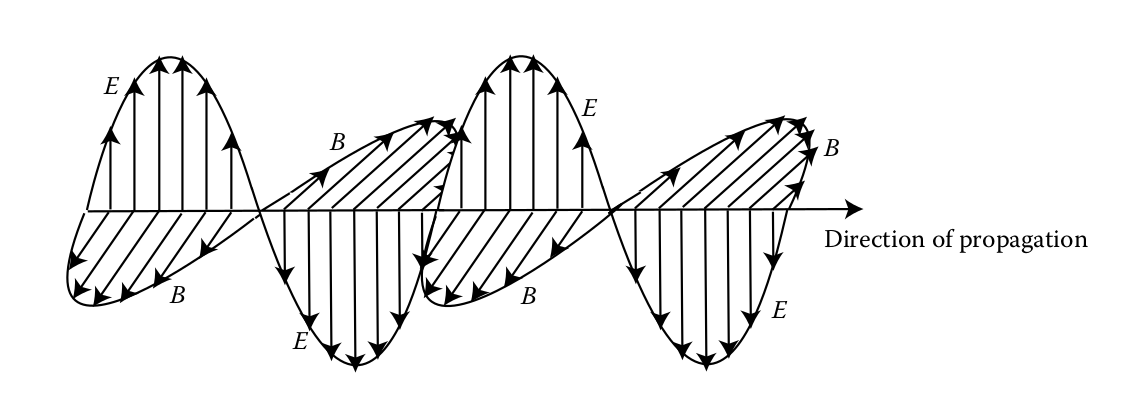
\includegraphics[width=0.7\textwidth]{Images/em_waves.png}
    \caption{Waves of electromagnetic radiation.}
    \label{fig:em_waves}
\end{figure}

The speed of EM waves in a vacuum is the speed of light, $c = 299 792 458$ m/s. The frequency, $\nu$, in hertz (Hz), and the wavelength, $\lambda$, in meters, are related by

\begin{equation}
    \lambda \nu = c
\end{equation}

EM waves are often generated by accelerating charged particles, typically electrons due to their smaller mass compared to protons. Light can be described both as a wave and as a particle (photon). The energy of a photon is given by

\begin{equation}
    E = h\nu = \frac{hc}{\lambda}
\end{equation}

where $h$ is Planck’s constant, $h = 6.626 \times 10^{-34}$ J s. The electromagnetic spectrum covers a wide range of frequencies and wavelengths (Figure~\ref{fig:em_spectrum}).

\begin{figure}[H]
    \centering
    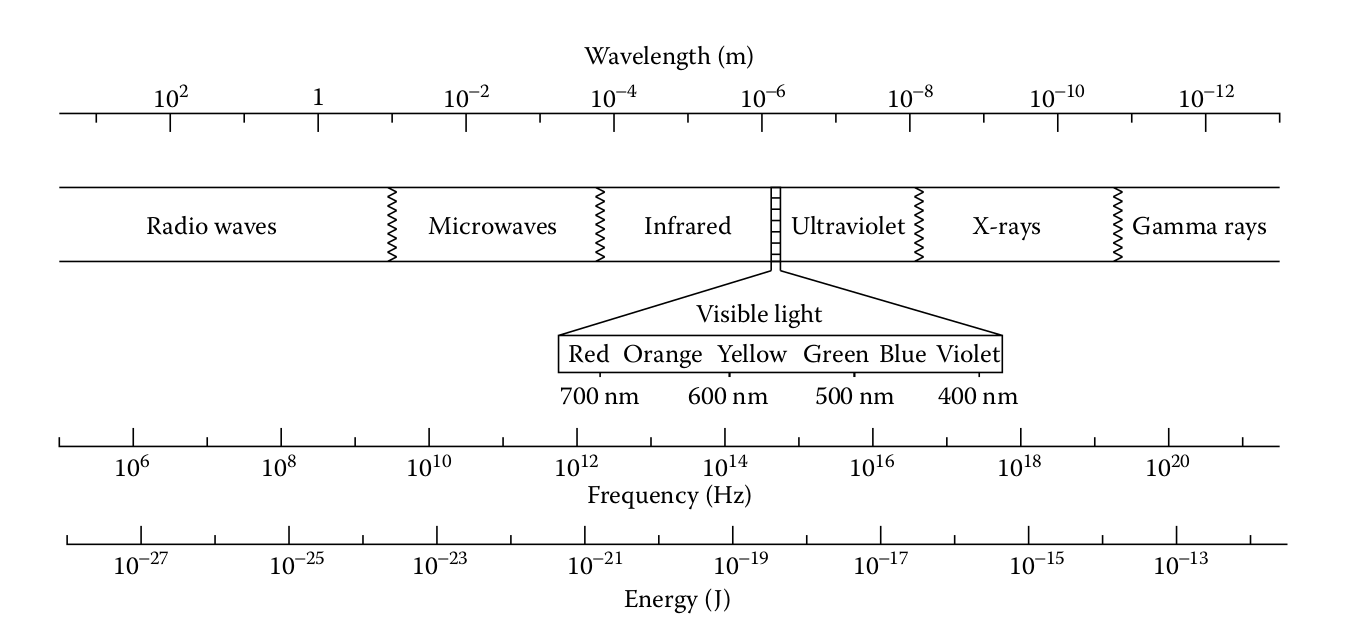
\includegraphics[width=0.7\textwidth]{Images/em_spectrum.png}
    \caption{The electromagnetic spectrum.}
    \label{fig:em_spectrum}
\end{figure}

The radio band spans from 10 MHz to 300 GHz (30 m to 1 mm in wavelength). The Earth's atmosphere allows radio waves within this range to reach the surface, except at very low frequencies (below 10 MHz) and high frequencies (above 300 GHz) due to ionospheric and atmospheric absorption.

\subsection{Spectroscopy}

Spectroscopy involves analyzing the spectrum (intensity vs. frequency or wavelength) of detected radiation, providing valuable information about the source. Classical spectrographs use prisms or gratings to separate wavelengths (Figure~\ref{fig:spectrograph}).

\begin{figure}[H]
    \centering
    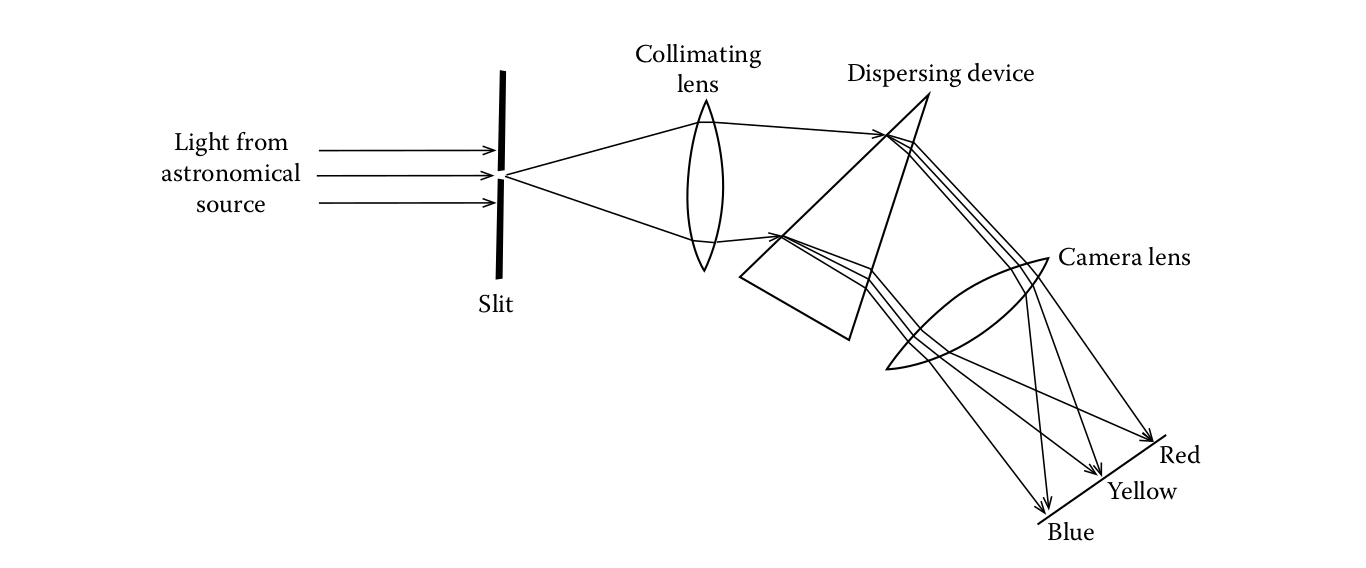
\includegraphics[width=0.7\textwidth]{Images/spectrograph.png}
    \caption{A classical spectrograph setup.}
    \label{fig:spectrograph}
\end{figure}

Radio spectrographs separate frequencies electronically, displaying the spectrum as intensity vs. frequency. There are three types of spectra based on Kirchhoff’s rules:

\begin{enumerate}
    \item \textbf{Continuous spectra:} Emission at all frequencies without breaks. An example is an incandescent lamp (Figure~\ref{fig:continuous_spectrum}).

    \begin{figure}[H]
        \centering
        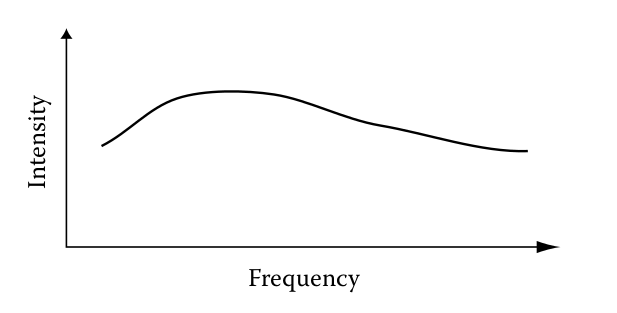
\includegraphics[width=0.7\textwidth]{Images/continuous_spectrum.png}
        \caption{Qualitative example of a continuous spectrum.}
        \label{fig:continuous_spectrum}
    \end{figure}

    \item \textbf{Emission line spectra:} Emission at specific frequencies due to quantum transitions in atoms or molecules (Figure~\ref{fig:emission_spectrum}).

    \begin{figure}[H]
        \centering
        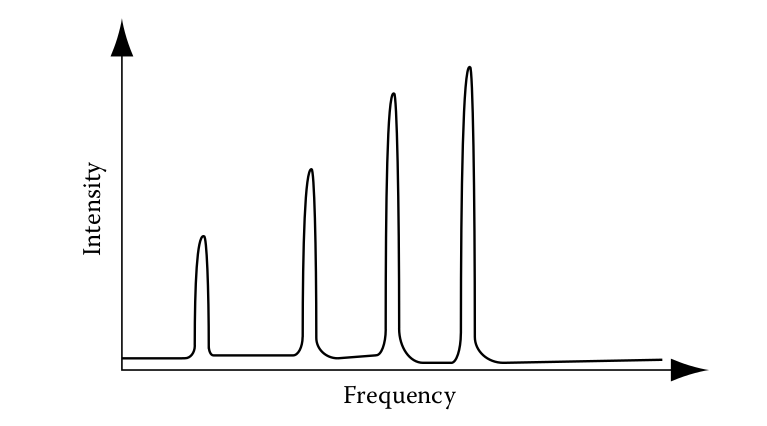
\includegraphics[width=0.7\textwidth]{Images/emission_spectrum.png}
        \caption{Qualitative sketch of an emission line spectrum.}
        \label{fig:emission_spectrum}
    \end{figure}

    \item \textbf{Absorption line spectra:} Dark lines appear when radiation passes through a cooler gas, which absorbs specific frequencies (Figure~\ref{fig:absorption_spectrum}).

    \begin{figure}[H]
        \centering
        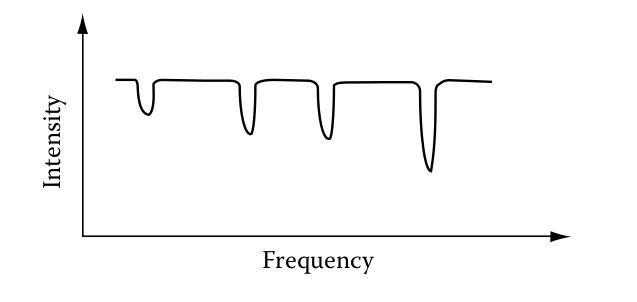
\includegraphics[width=0.7\textwidth]{Images/absorption_spectrum.png}
        \caption{Qualitative example of an absorption line spectrum.}
        \label{fig:absorption_spectrum}
    \end{figure}
\end{enumerate}

The specific frequencies of emission and absorption lines allow identification of the chemical composition of the source or intervening gas.

\clearpage

\section{Sky Coodinate System}

\subsection{Right Ascension and Declination}
To locate objects in the sky, we use a coordinate system similar to Earth's. The celestial sphere, an imaginary globe surrounding Earth, uses extensions of longitude (right ascension, RA, $\alpha$) and latitude (declination, Dec, $\delta$) lines. The celestial poles align with Earth's poles, and the sky appears to rotate about an axis through these poles.

\begin{figure}[H]
    \centering
    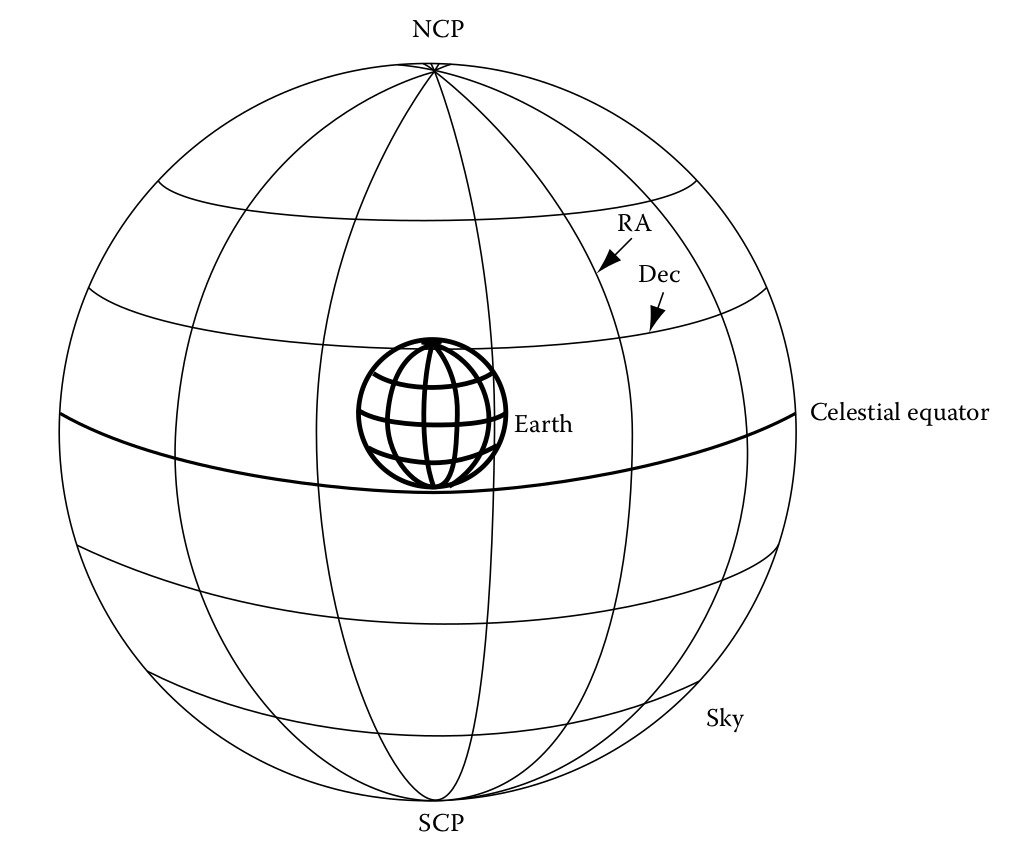
\includegraphics[width=0.7\textwidth]{Images/ra_dec.png}
    \caption{The celestial sphere with RA and Dec lines.}
    \label{fig:ra_dec}
\end{figure}

Declination is analogous to latitude and is measured in degrees from the celestial equator. RA, fixed relative to the stars, is defined such that the $0^\circ$ line of RA aligns with the $0^\circ$ line of longitude at noon on the first day of spring. RA is measured in hours, minutes, and seconds, with $24\,h$ of RA corresponding to $360^\circ$. \\

The units of RA are time-based due to historical reasons and simplify calculations involving Earth's rotation. The conversion between RA and degrees at the equator is $1\,h$ RA = $15^\circ$ arc, $1\, \min$ RA = $15\, \min$ arc, and $1\,s$ RA = $15\,s$ arc. Away from the equator, the angular separation between RA lines depends on declination ($\delta$) and is given by:
\[
\text{Seconds of arc} = 15 \cos (\delta) \times \text{seconds of RA}
\]

On sky maps, east appears to the left, and RA increases to the left, due to the observer's perspective relative to the ground.

\subsection{Observer-Centered Definitions}
\begin{enumerate}
    \item \textbf{Horizon}: The boundary of visible sky, blocked by the ground.
    \item \textbf{Zenith}: The point directly overhead.
    \item \textbf{Altitude/Elevation}: Angular height above the horizon ($0^\circ$ at horizon, $90^\circ$ at zenith).
    \item \textbf{Azimuth}: Angular position along the horizon from north ($0^\circ$ north, $180^\circ$ south, $90^\circ$ east, $270^\circ$ west).
    \begin{figure}[H]
        \centering
        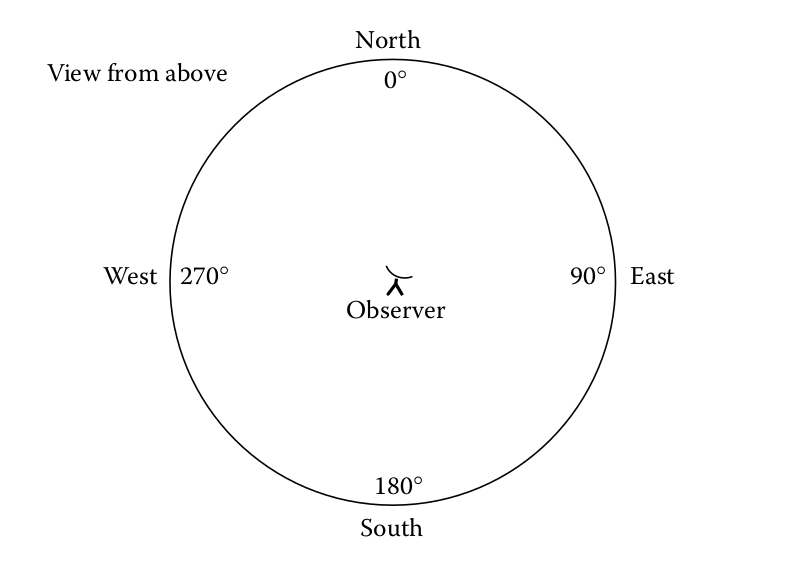
\includegraphics[width=0.7\textwidth]{Images/azimuthal_angles.png}
        \caption{View from above depicting azimuthal angles along with the cardinal directions around the horizon.}
        \label{fig:azimuthal_angles}
    \end{figure}
    \item \textbf{Meridian}: The line of RA through your zenith, connecting to celestial poles.
    \begin{figure}[H]
        \centering
        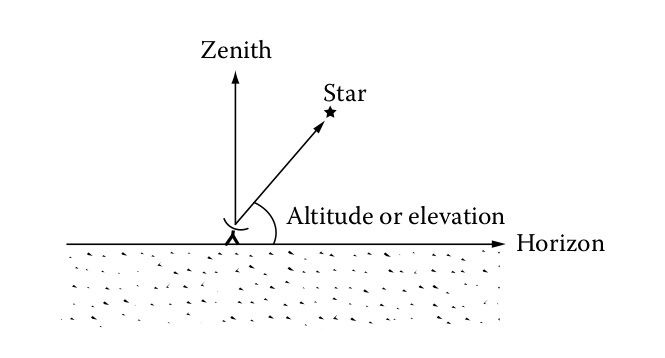
\includegraphics[width=0.7\textwidth]{Images/zenith_horizon_altitude_elevation.png}
        \caption{Schematic diagram showing the relations between zenith, horizon, and altitude or elevation.}
        \label{fig:zenith_horizon_altitude_elevation}
    \end{figure}
    \item \textbf{Transit}: When an object crosses your meridian, highest in the sky.
    \item \textbf{Hour Angle (HA)}: Hours since an object crossed your meridian.
    \item \textbf{Local Sidereal Time (LST)}: RA currently on your meridian, running slightly faster than solar time. (HA = LST - RA)
    \item \textbf{Universal Time (UT)}: Local solar time at Greenwich, England, standardized for timekeeping.
\end{enumerate}

RA measured in time simplifies finding when objects cross the meridian and explains its increase to the east.

\begin{figure}[H]
    \centering
    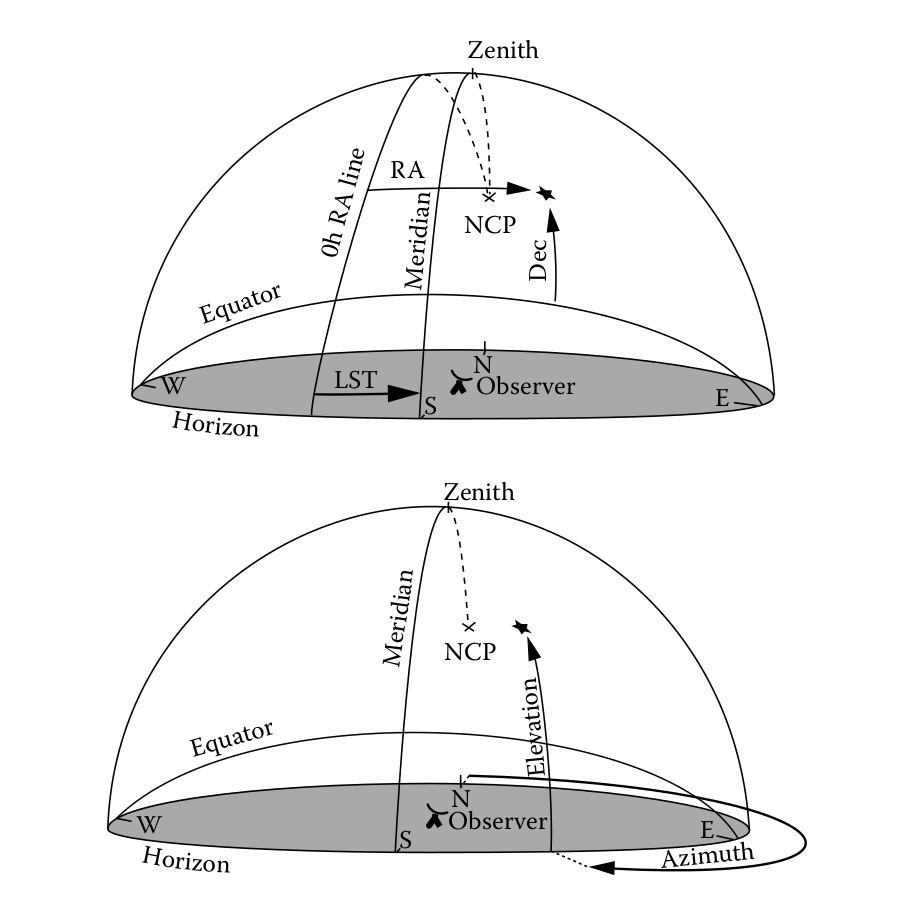
\includegraphics[width=0.7\textwidth]{Images/sky_coordinates_example.png}
    \caption{Example of sky coordinates as viewed by the observer (top) and observer-centered coordinates (bottom).}
    \label{fig:sky_coordinates_example}
\end{figure}

\subsection{Apparent Sizes}
Angular size, dependent on an object's actual size and distance, is measured in radians:
\[
\theta \, (\text{radians}) = \frac{s}{r}
\]
For small angles:
\[
\theta \, (\text{radians}) \approx \frac{l}{d}
\]
In two dimensions, the solid angle $\Omega$ is:
\[
\Omega = \frac{A}{d^2}
\]
with the unit steradian (sr), and the whole sky covering $4\pi$ sr.

Understanding these coordinate systems allows us to locate and observe celestial objects from any Earth location and describe their apparent positions and sizes accurately.


\clearpage

\section{Radio Telescopes}

Observing with a radio telescope differs significantly from using a visible-wavelength telescope. The Sun does not illuminate the entire sky at radio wavelengths, resulting in a dark daytime sky suitable for observations day and night. Long radio wavelengths penetrate clouds, whereas shorter wavelengths require clear skies due to water-induced signal loss. \\

A traditional radio telescope comprises five basic parts.

\begin{figure}[H]
    \centering
    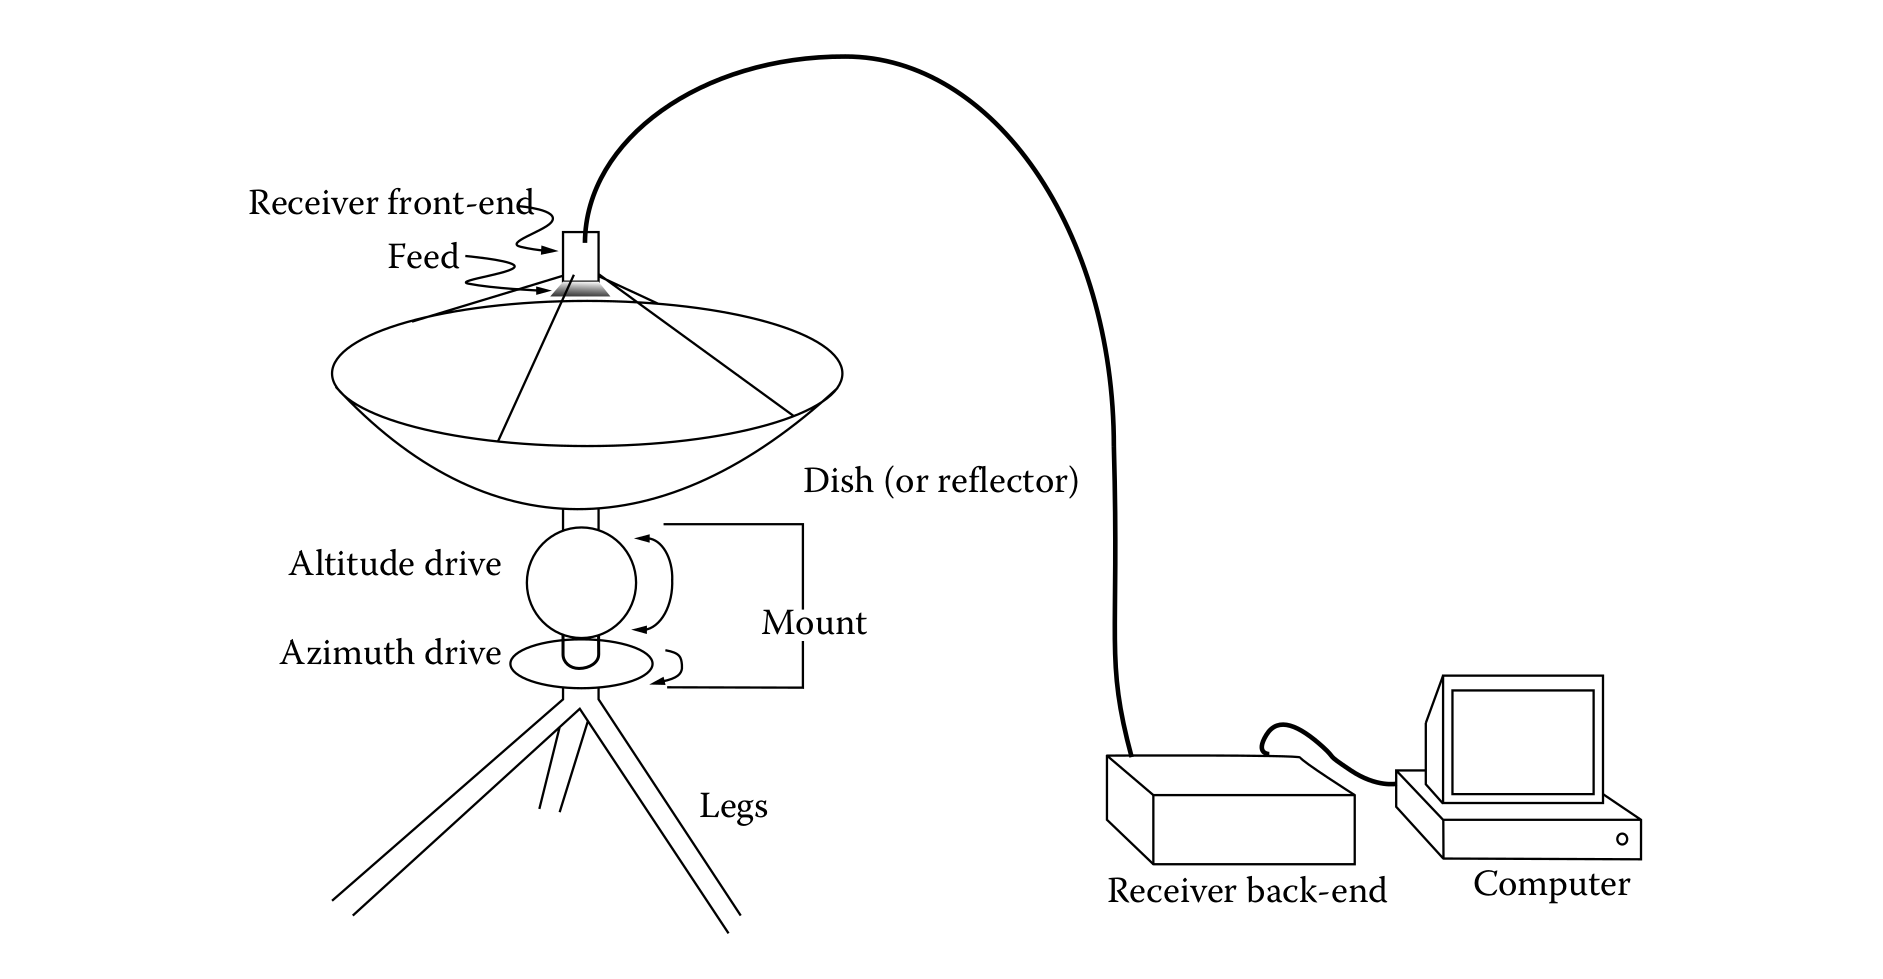
\includegraphics[width=0.5\textwidth]{Images/radio_telescope.png}
    \caption{A schematic diagram of a radio telescope.}
    \label{fig:radio_telescope}
\end{figure}

\subsection{Parabolic Reflector}
Most radio telescopes use a parabolic reflector (dish) to collect and focus radio waves. Unlike visible-light telescopes, radio telescopes do not use lenses. The radiation can be detected at the focal point (prime focus) or behind the dish (Cassegrain focus).

\begin{enumerate}
    \item The sensitivity of the telescope depends on the collecting area, proportional to the square of the reflector's diameter.
    \item Radio dishes do not need highly polished surfaces. Successful reflection occurs when surface irregularities are much smaller than the wavelength, \(\delta z < \frac{\lambda}{20}\). For longer wavelengths, the surface can be a mesh.
    \item The resolution of a radio telescope is determined by diffraction, improving with larger reflectors.
\end{enumerate}

\subsection{Mount}
The mount holds and moves the dish, allowing rotation around two axes. Modern radio telescopes use altitude-azimuth (Alt-Az) mounts, while older visible-wavelength telescopes often use equatorial mounts.

\subsection{Feeds, Receivers, and Computer}
The dish focuses radio waves to feeds that convert them into transmission lines, sending signals to receivers. The receiver front-end amplifies and processes the signal, which is then transmitted to the observatory's control room for further processing by the back-end and storage on a computer. \\

Each feed-receiver assembly acts like a pixel. Radio telescopes typically have fewer feed-receiver assemblies compared to the megapixel arrays in visible-wavelength telescopes due to the larger size and cost. Large telescopes like Arecibo and Green Bank can have 7 to 13 assemblies, while smaller ones like Haystack SRT have only one. At millimeter wavelengths, arrays with thousands of bolometer detectors exist. \\

Radio observations often yield fewer data points compared to visible-wavelength observations, but aperture synthesis (combining signals from multiple telescopes) can produce detailed images.

\clearpage

\section{Radio Maps}

Displaying the structure of a source at radio wavelengths requires choosing the best way to present two-dimensional data. There are three common approaches:

\subsection{Contour Maps}

The simplest way is using a contour map, where contours are lines of constant intensity, similar to a topographical map indicating lines of constant elevation. Closely spaced contours indicate regions where the intensity changes rapidly. An example of a contour map is shown in Figure~\ref{fig:contour_map}.

\begin{figure}[H]
    \centering
    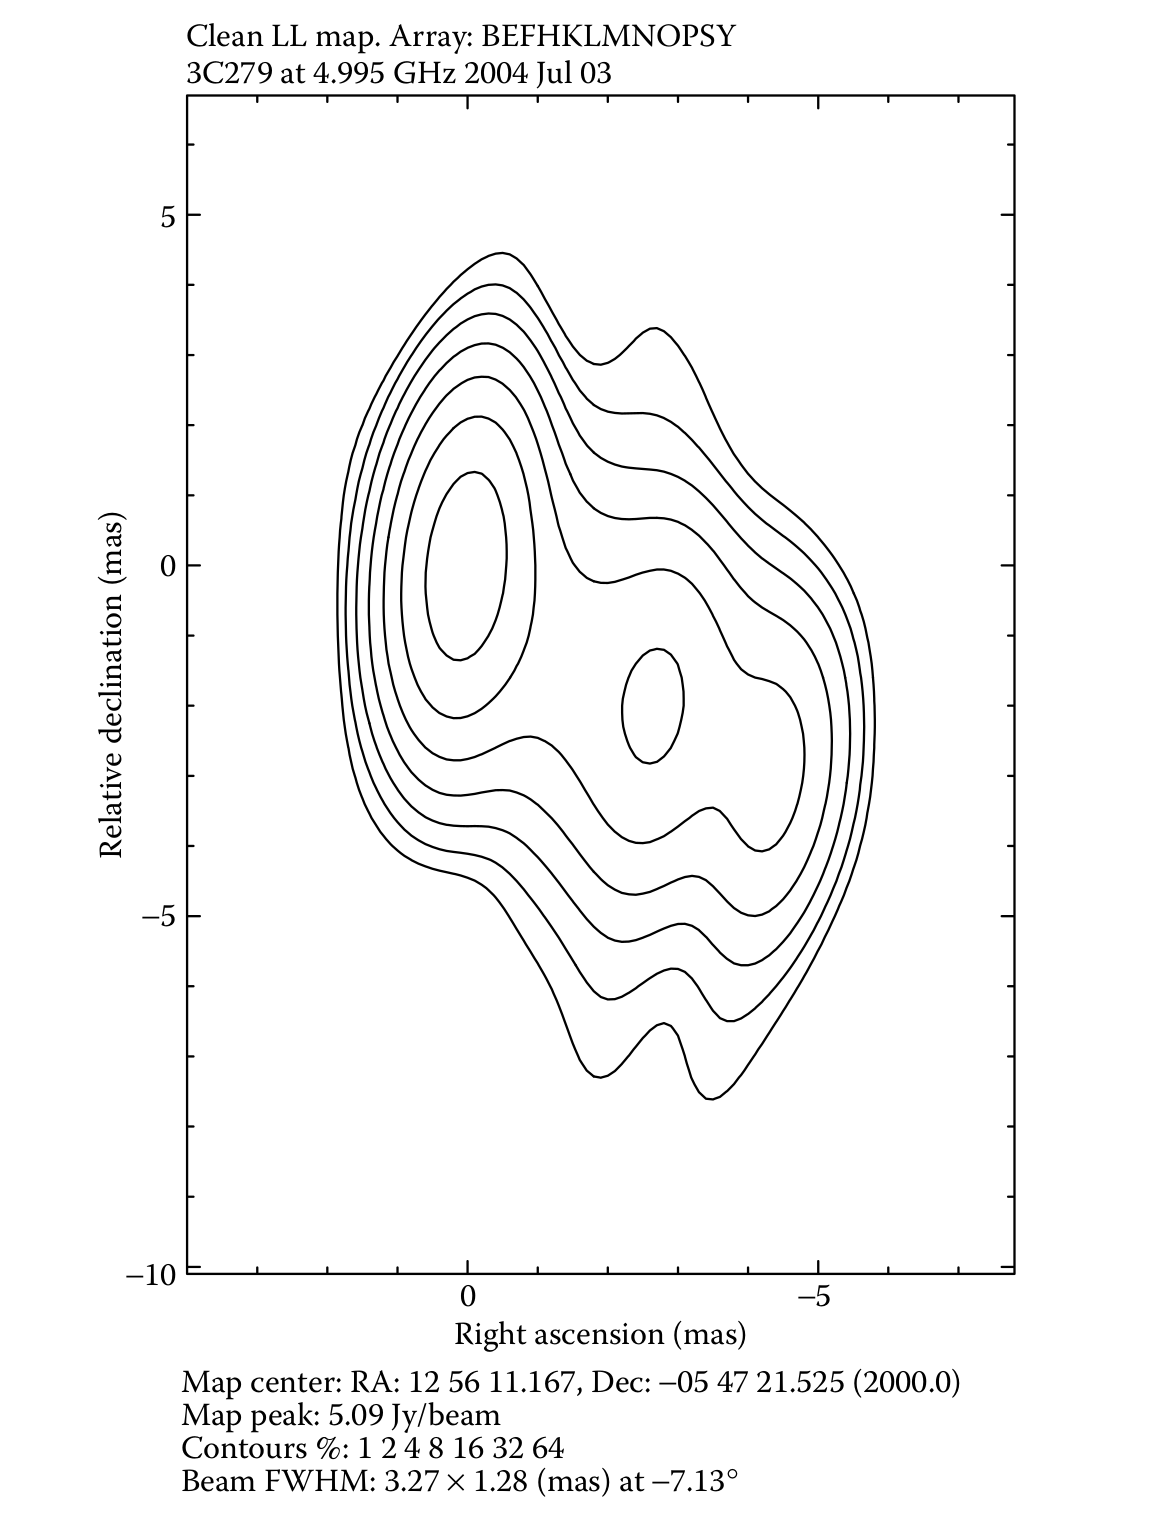
\includegraphics[width=0.7\textwidth]{Images/contour_map.png}
    \caption{An example of a contour map.}
    \label{fig:contour_map}
\end{figure}

\subsection{Gray Scale Maps}

A gray scale map directly indicates brightness variations with shades of gray, where black is the most intense and white the least. Although gray scale maps are more intuitive, they often do not reveal details as well as contour maps. Therefore, contour maps are preferred for detailed analysis. Overlaid gray scale and contour maps, as shown in Figure~\ref{fig:gray_scale_contour_overlay}, are common and visually pleasing.

\begin{figure}[H]
    \centering
    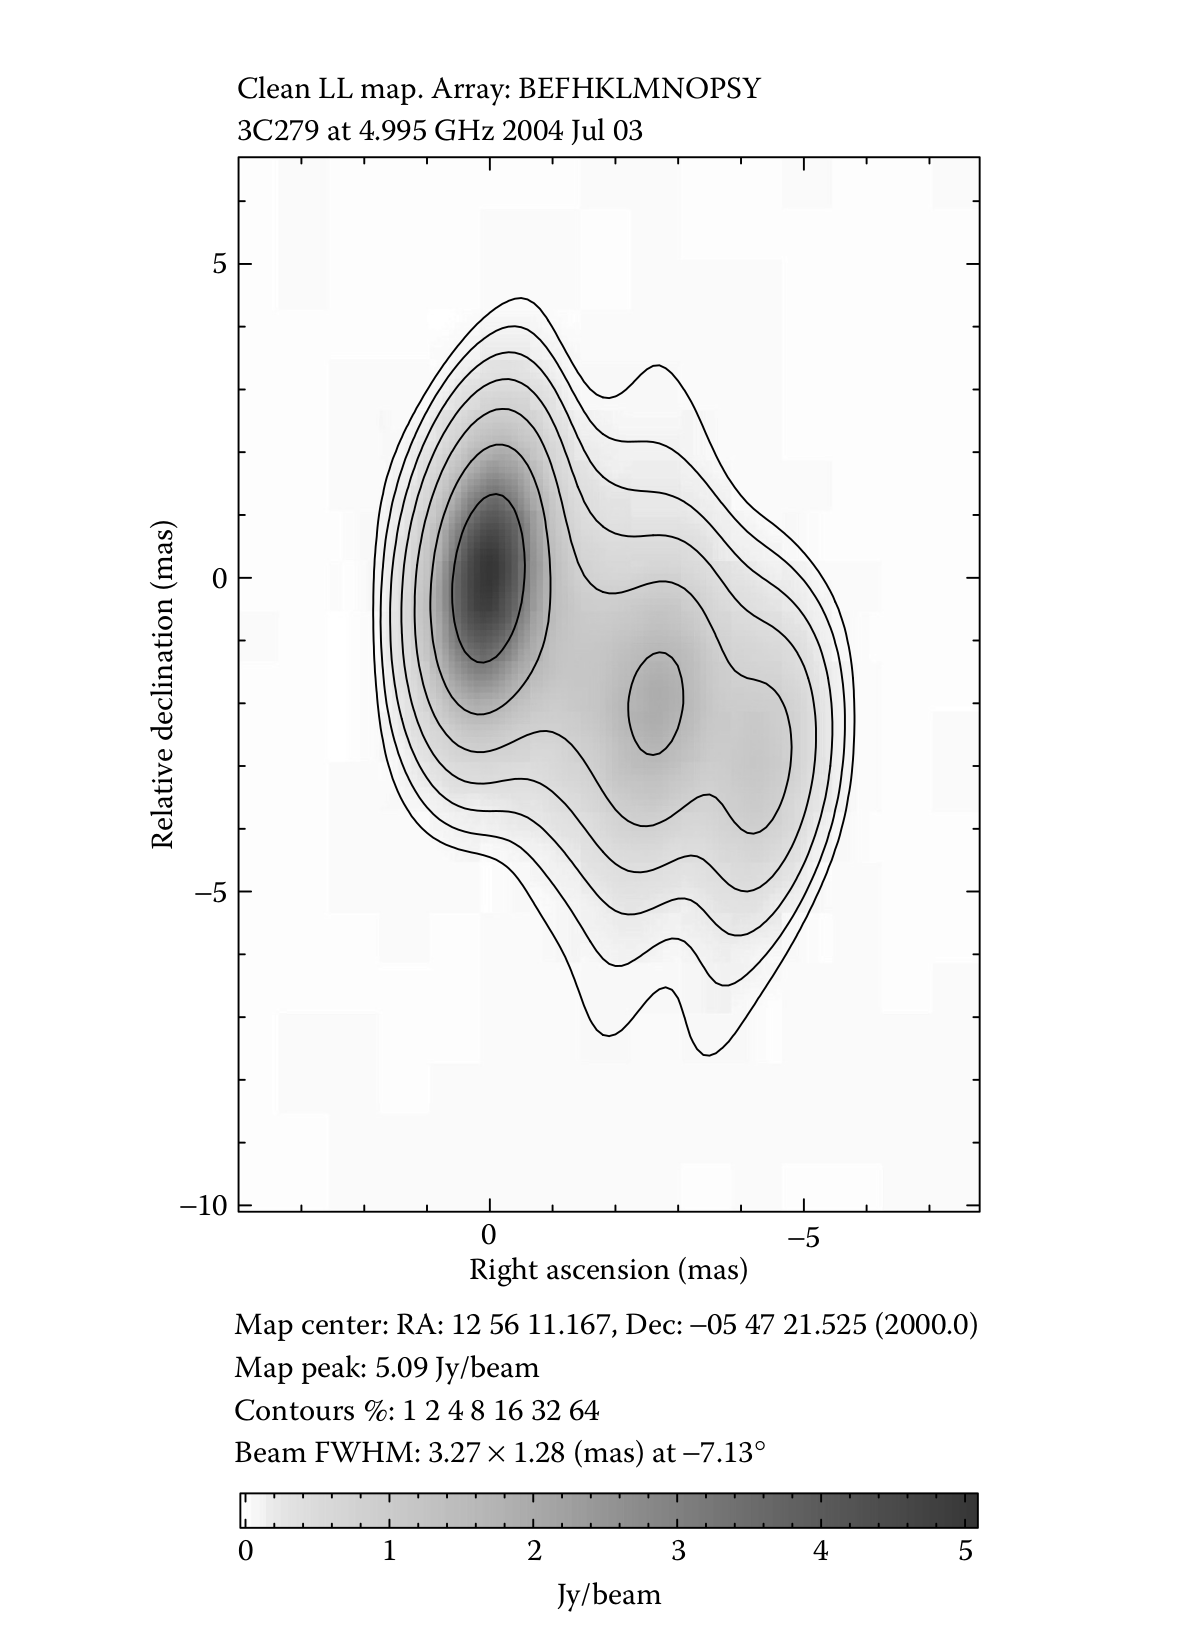
\includegraphics[width=0.7\textwidth]{Images/gray_scale_contour_overlay.png}
    \caption{An example of an overlaid gray scale and contour map.}
    \label{fig:gray_scale_contour_overlay}
\end{figure}

\subsection{False Color Maps}

False color maps use colors to indicate different levels of brightness rather than wavelengths. These images often include a color-wedge to show the relationship between color and brightness, facilitating analysis. An example of a false color map is shown in Figure~\ref{fig:false_color_map}.

\begin{figure}[H]
    \centering
    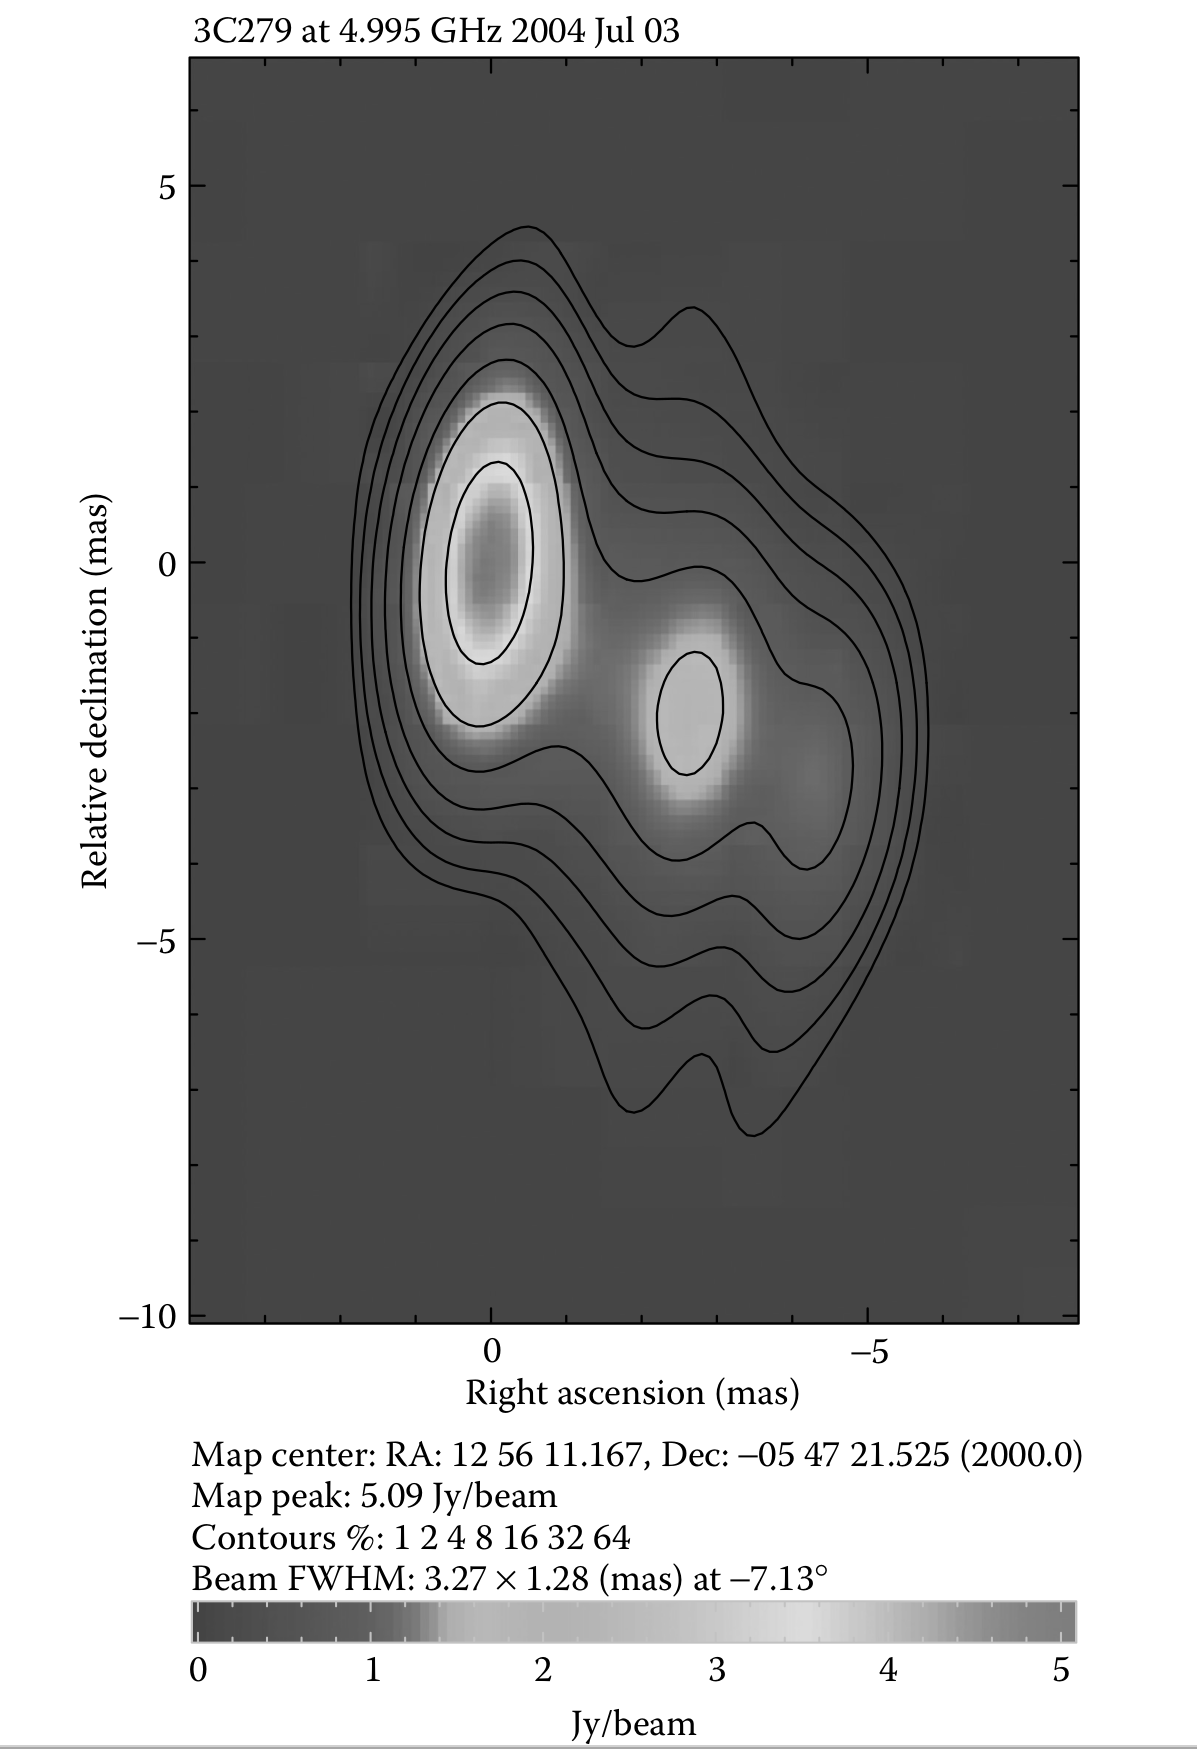
\includegraphics[width=0.6\textwidth]{Images/false_colour_map.png}
    \caption{An example of a false color map.}
    \label{fig:false_color_map}
\end{figure}

\subsection{Multicolor Images}

Radio astronomers sometimes create multicolor images similar to visible light astronomers. By observing several different radio wavelengths, images can be overlaid, assigning red to the longest wavelength, green to intermediate wavelengths, and blue to the shortest wavelength.


\clearpage

\section{Galaxy FITS Data in Multiple Wavelengths}

We will choose 3 Galaxies - Sunflower, Tadpole and Whirlpool Galaxy, and use the CIRADA \cite{cirada_cutout} image cutout web service to display their FITS\cite{fits_nasa} data in multiple wavelengths. This service enables us to obtain optical, infrared, and radio images of all three galaxies.

Different wavelengths reveal different aspects of the galaxies. Optical images show the distribution of stars, while infrared images reveal the distribution of dust and gas. Radio images show the distribution of cold gas and synchrotron radiation from cosmic rays.

\subsection{Sunflower Galaxy}

\begin{figure}[H]
    \centering
    \includegraphics[width=\textwidth]{Images/sunflower.png}
    \caption{Sunflower Galaxy in multiple wavelengths.}
    \label{fig:sunflower}
\end{figure}

\subsection{Tadpole Galaxy}
    
\begin{figure}[H]
    \centering
    \includegraphics[width=\textwidth]{Images/tadpole.png}
    \caption{Tadpole Galaxy in multiple wavelengths.}
    \label{fig:tadpole}
\end{figure}

\subsection{Whirlpool Galaxy}

\begin{figure}[H]
    \centering
    \includegraphics[width=\textwidth]{Images/whirlpool.png}
    \caption{Whirlpool Galaxy in multiple wavelengths.}
    \label{fig:whirlpool}
\end{figure}

\clearpage

\section{Jet Afterglow Lightcurve of GW170817}

GW170817\cite{gw170817_afterglow} was a merger of two neutron stars that was accompanied by both gravitational waves and electromagnetic radiation. We used the data for the non-thermal emission from this source that spans across all frequency bands following a single spectral index of $F_{\nu} \propto {\nu}^{-0.584}$ . The quantity F is the flux density, which measures the amount of energy incident on the detector per unit area of the detector, an indicator of the brightness of the source. A lightcurve is this flux density represented as a function of time. \\

We plotted the lightcurve choosing all the VLA 3 GHz data points.

\begin{figure}[H]
    \centering
    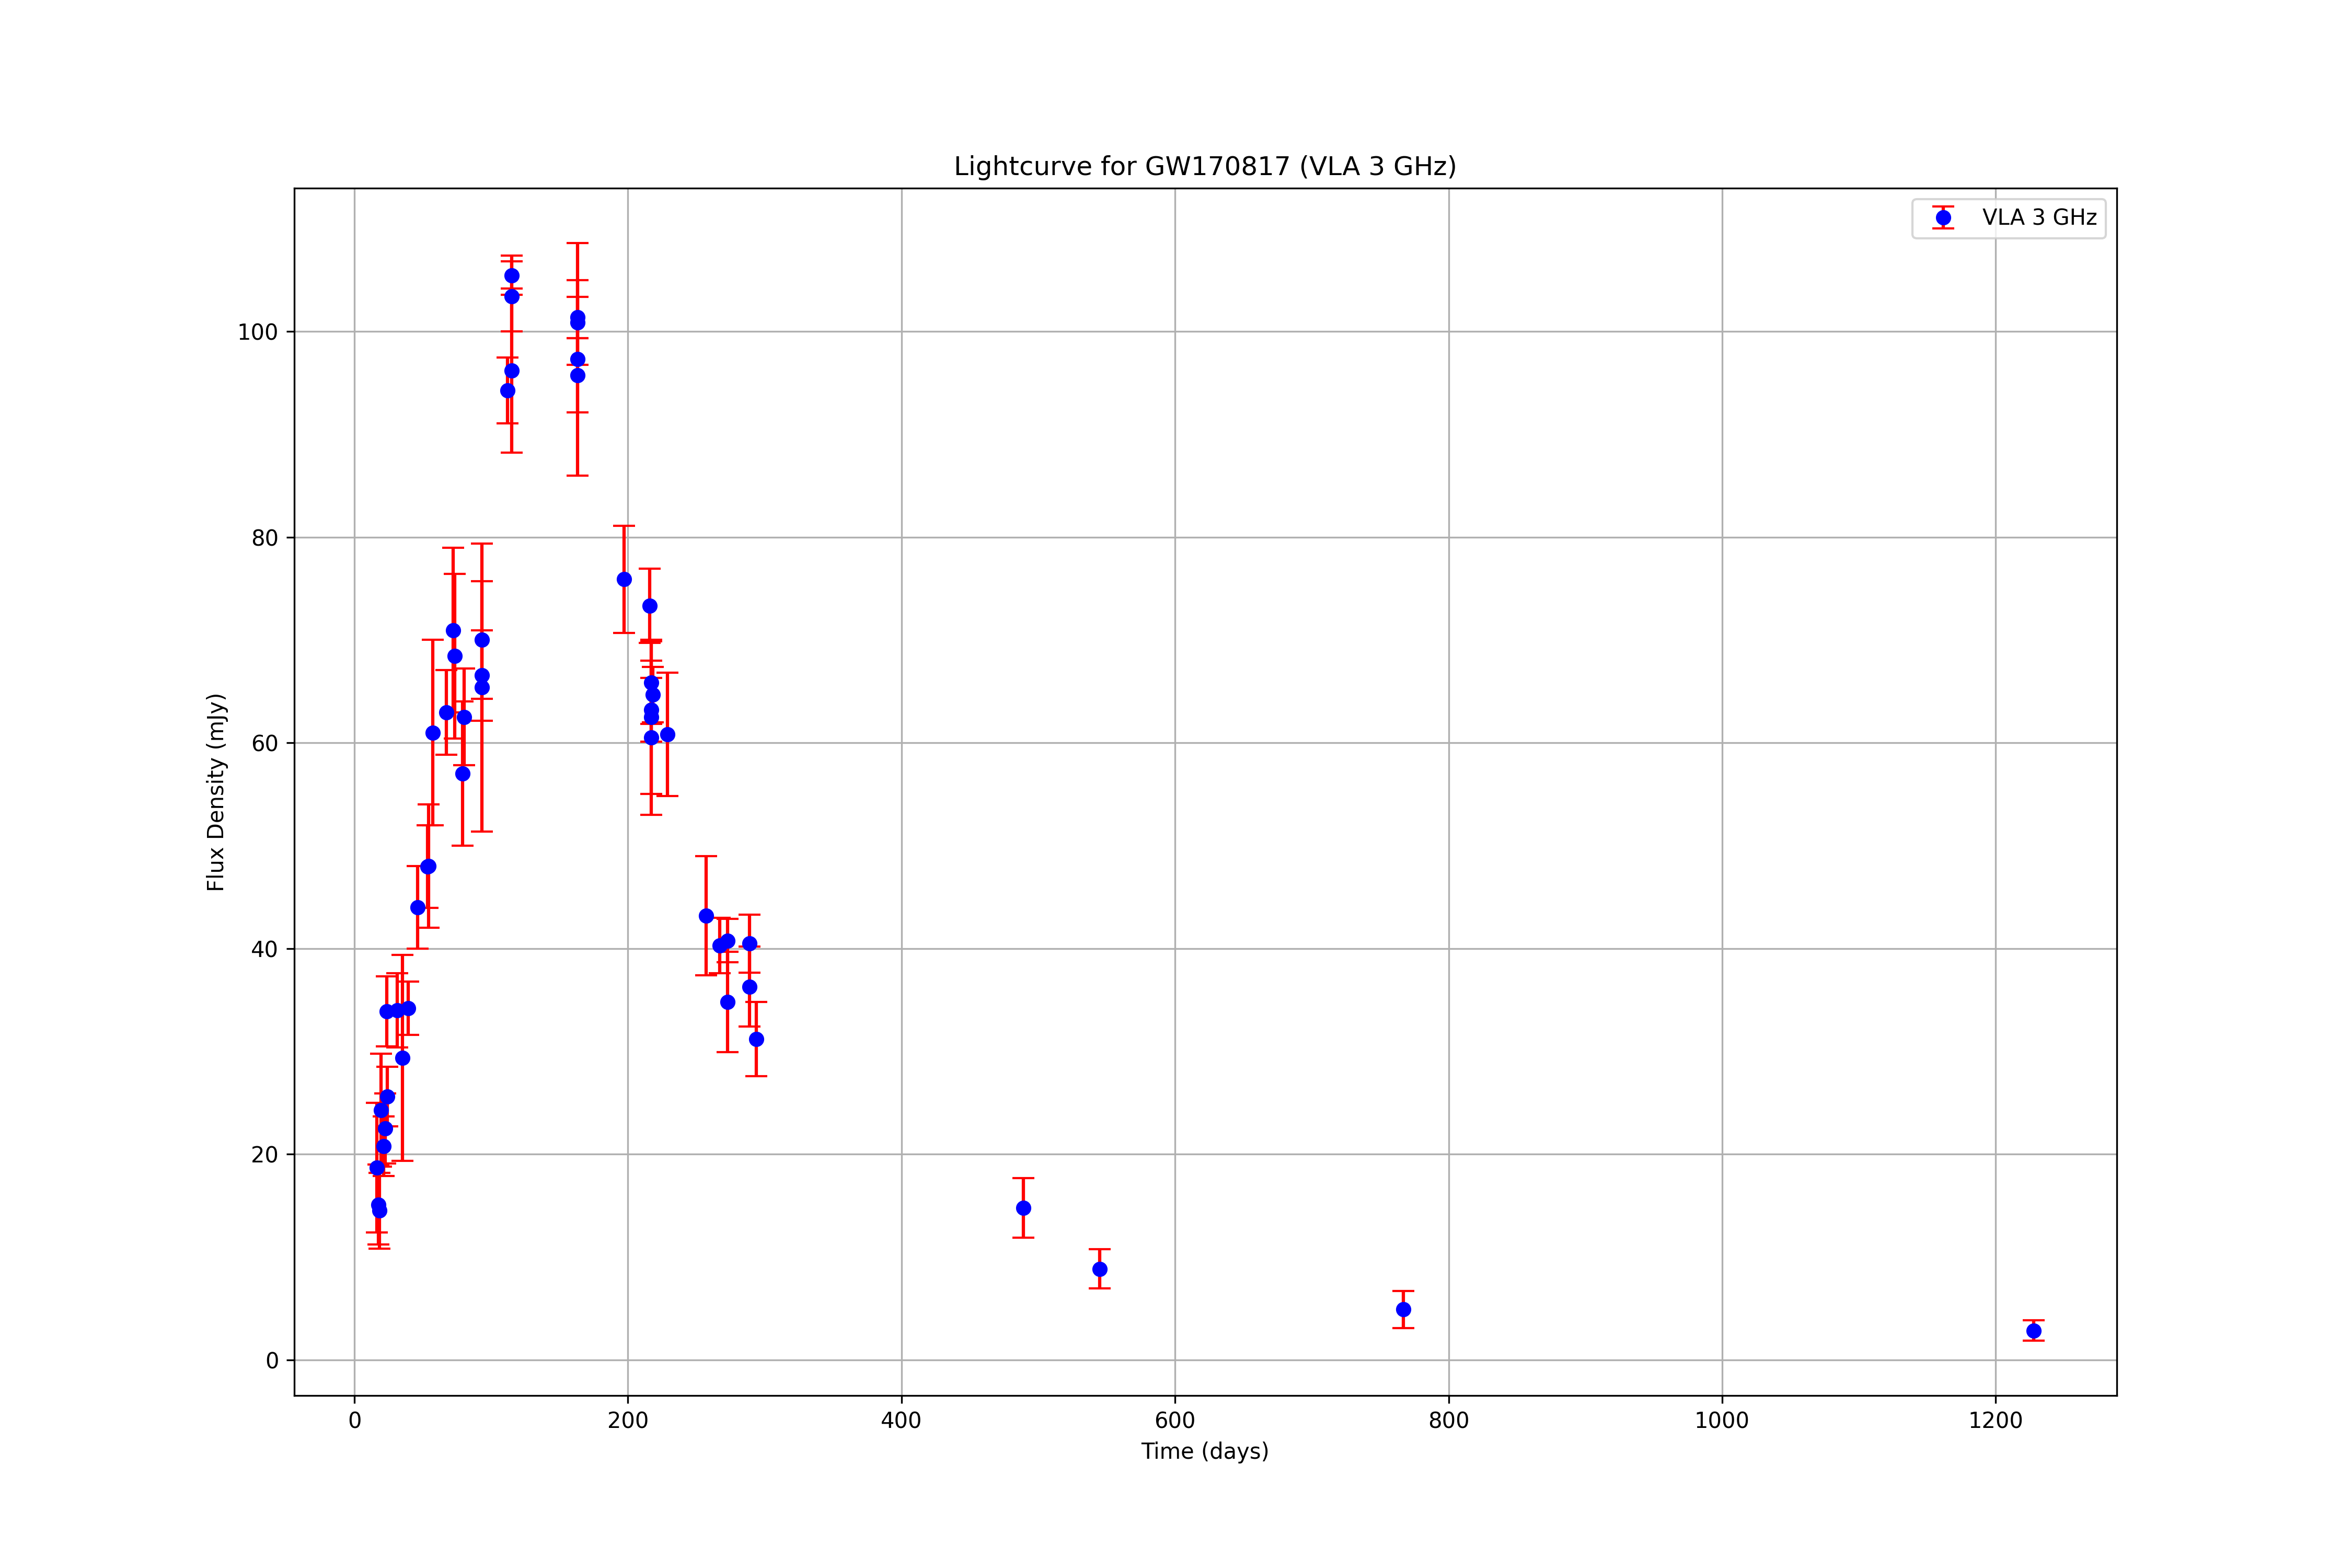
\includegraphics[width=0.6\textwidth]{Images/vla_lightcurve.png}
    \caption{Flux Density vs Time at 3GHz frequency measured by VLA telescope.}
    \label{fig:vla_lightcurve}
\end{figure}

\vspace{10mm}

We also plotted the lightcurve choosing all the Chandra 3 GHz data points.

\begin{figure}[H]
    \centering
    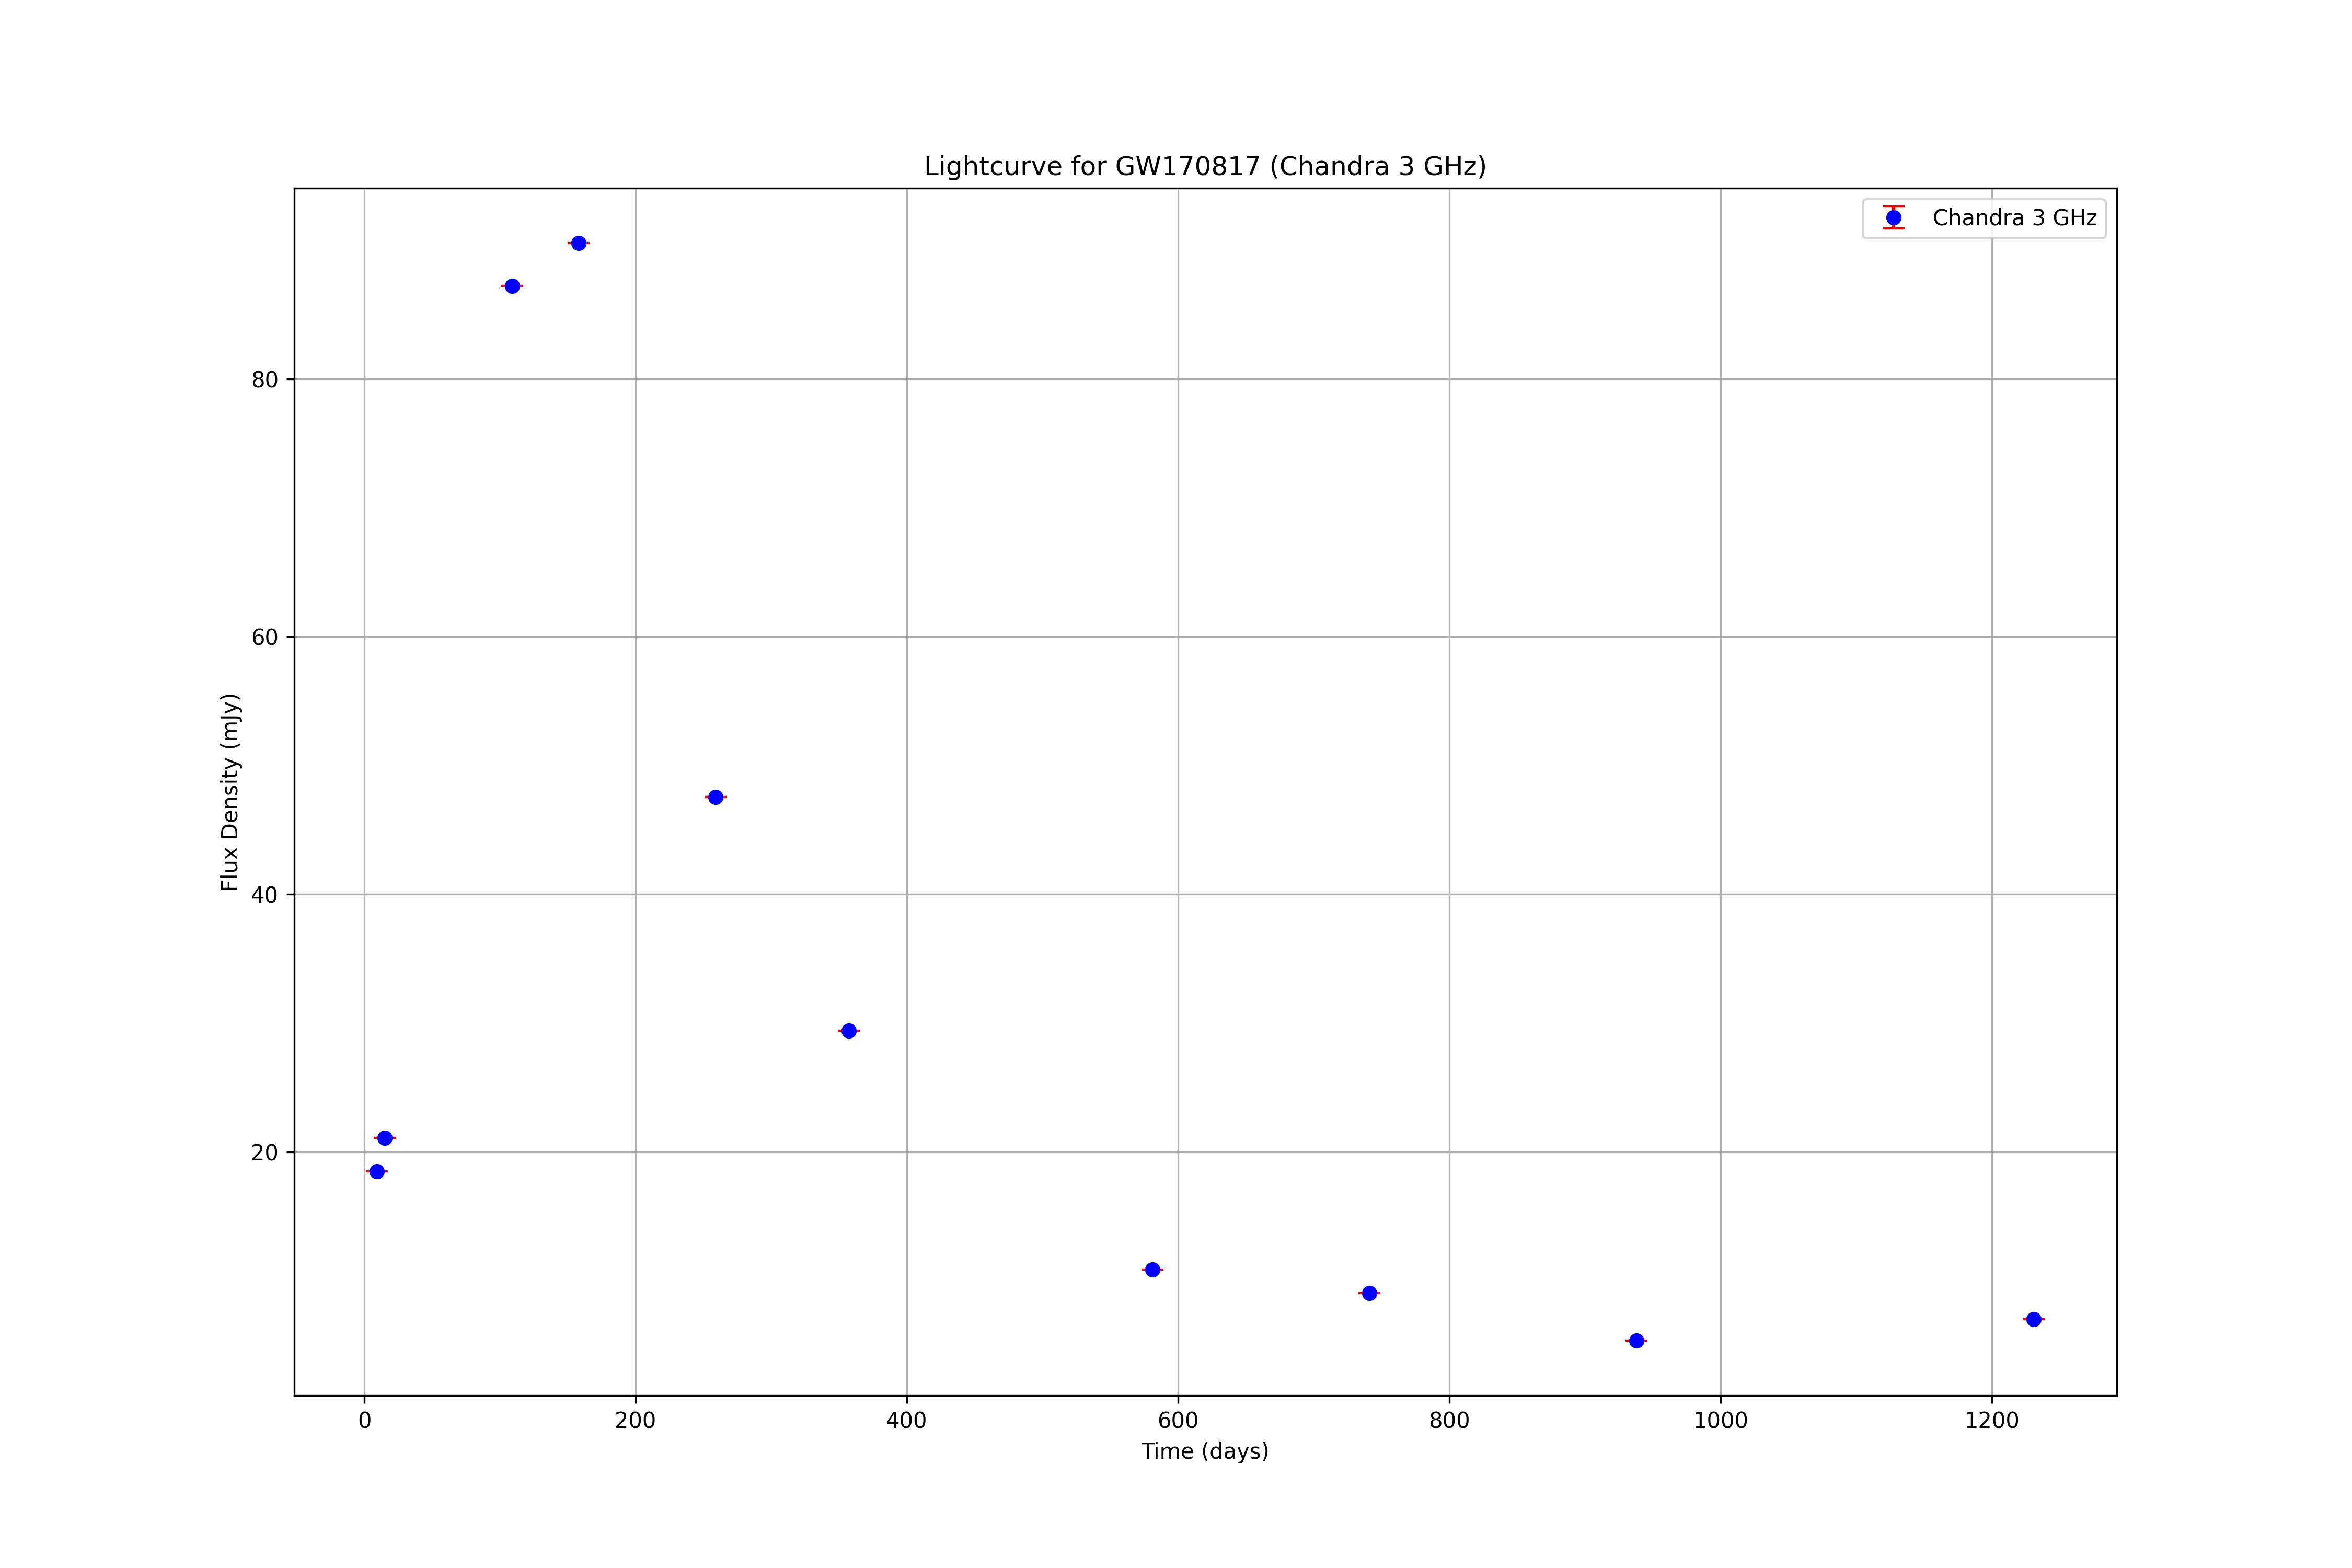
\includegraphics[width=0.6\textwidth]{Images/chandra_lightcurve.png}
    \caption{Flux Density vs Time at 3GHz frequency measured by Chandra telescope.}
    \label{fig:chandra_lightcurve}
\end{figure}


\chapter{Introduction to Radiation Physics}

\section{Measuring Radiation}

One quantitative measure that astronomers use when observing a light source is the amount of radiation received. Quantifying this amount involves several related but distinct concepts. We discuss these measures below.

\subsection{Total Energy Emitted}

A source's total light output can be described by the total amount of energy emitted over its lifetime, at all frequencies, and in all directions. However, this comprehensive measure is impractical for direct observation since we can only measure radiation over finite time periods. Instead, we focus on measurements normalized by time.

\subsection{Luminosity}

Luminosity (L) or power is the rate at which energy is emitted by a source, expressed in watts (W) or ergs per second (erg s\textsuperscript{-1}). It is calculated by dividing the total emitted energy by the time period over which it was emitted.

\subsection{Flux}

Flux (F) measures the amount of light energy per unit time per unit area that we detect from a source. It is normalized by dividing the detected power by the effective area of the telescope receiving the radiation. Flux is expressed in units of joules per second per square meter (J s\textsuperscript{-1} m\textsuperscript{-2}) or watts per square meter (W m\textsuperscript{-2}).

The relationship between flux and luminosity for an isotropic source at distance \( d \) is given by:
\[ F = \frac{L}{4 \pi d^2} \]

\subsection{Flux Density}

Flux density ($F_{\nu}$ or $F_{\lambda}$) refers to the flux per unit frequency or wavelength range observed. It is calculated by dividing the detected flux by the frequency or wavelength bandwidth (\( \Delta \nu \) or \( \Delta \lambda \)). Flux density is crucial in characterizing the spectral properties of sources.

For radio astronomy, flux density per unit frequency (\( S_{\nu} \)) in janskys (Jy) is a commonly used unit:
\[ 1 \text{ Jy} = 10^{-26} \text{ W m}^{-2} \text{ Hz}^{-1} \]

\subsection{Intensity}

Intensity $I_{\nu}$ or $I_{\lambda}$, also known as specific intensity or surface brightness, is the flux density per unit solid angle. It measures the amount of energy radiated per second per unit area per unit solid angle of the source. Intensity is independent of distance and provides insights into the microscopic radiation processes of the emitting object.

The relationship between flux density and intensity is:
\[ I_\nu = \frac{F_\nu}{\Omega} \]

where \( \Omega \) is the solid angle subtended by the source. Intensity is commonly expressed in units of watts per square meter per hertz (W Hz\textsuperscript{-1} m\textsuperscript{-2} sr\textsuperscript{-1}) or watts per square meter per nanometer (W nm\textsuperscript{-1} Hz\textsuperscript{-1} m\textsuperscript{-2} sr\textsuperscript{-1}) depending on the wavelength regime.

\subsection{Relation between Intensity and Electric Field}

Intensity is related to the electric field strength of the radiation waves via the Poynting vector. The intensity of radiation is proportional to the square of the electric field amplitude \( E_0 \).

\[ I_\nu \propto E_0^2 \]

This relationship underscores the fundamental connection between the electromagnetic wave properties and the measurable quantities of radiation intensity.

In summary, astronomers employ various measures such as luminosity, flux, flux density, and intensity to quantitatively describe the amount of radiation emitted by astronomical sources. Each measure provides unique insights into the nature and properties of celestial objects across different wavelength regimes.

\section{Blackbody Radiation}
\label{sec:blackbodyradiation}

At the start of the twentieth century, Max Planck's discovery that light's energy is quantized into packets called photons was pivotal. Blackbody radiation, the light emitted by a body that absorbs all incident light, is a key concept. This radiation helps us understand how hot objects cool by emitting light. \\

A blackbody is an idealized object that emits radiation solely based on its temperature, with no reflection or transmission. The interactions between photons and particles within the blackbody result in a thermal equilibrium, where both have the same temperature. \\

Photons are described by Bose–Einstein statistics, which help in determining the distribution of photon energies in thermal equilibrium. The energy distribution function of photons is directly related to the spectrum of emitted light, known as the Planck function:

\begin{equation}
	B_\nu (T) = \frac{2h\nu^3}{c^2} \frac{1}{e^{h\nu/kT} - 1}
	\label{eq:planckfunctionfrequency}
\end{equation}


where:
\begin{itemize}
    \item \(h = 6.626 \times 10^{-34} \, \text{J s} = 6.626 \times 10^{-27} \, \text{erg s}\) is Planck’s constant
    \item \(k = 1.38 \times 10^{-23} \, \text{J K}^{-1} = 1.38 \times 10^{-16} \, \text{erg K}^{-1}\) is Boltzmann’s constant
    \item \(c\) is the speed of light
    \item \(\nu\) is the frequency of the observation
    \item \(T\) is the temperature of the radiating body in Kelvins
\end{itemize}

In the Planck function given in Equation~\eqref{eq:planckfunctionfrequency}, written as $B_\nu(T)$, the subscript $\nu$ indicates that the spectral measure is per unit frequency and $B$ represents the intensity, or brightness, of the blackbody radiation and has units of intensity, \( \text{W m}^{-2} \text{Hz}^{-1} \text{sr}^{-1} \). Since this is an intensity, the Planck function can also be expressed as flux per unit wavelength per steradian, which is denoted as $B_\lambda(T)$. Radio astronomers generally express the Planck function using $B_\nu(T)$. The equation for $B_\lambda(T)$ is

\begin{equation}
	B_\lambda (T) = \frac{2hc^2}{\lambda^5} \frac{1}{e^{hc / \lambda k T} - 1}
	\label{eq:planckfunctionwavelength}
\end{equation}


It is very important to understand and appreciate that, even though \(B_\nu\) and \(B_\lambda\) represent the same concept, they are not the same numerical quantity or even the same function. We discuss in more detail about the difference between these functions later in this section. We first discuss some important features of the Planck function. \\

Figures~\ref{fig:planckfunctionnu} and~\ref{fig:planckfunctionlambda} display the log-log plots of these functions. Blackbody emission is a continuous spectrum that reaches zero at \(\nu = 0\) (owing to the \(\nu^3\) term), increases to some peak value as \(\nu\) increases, and then decreases and reaches zero again at \(\nu = \infty\) (owing to the exponential term). Note that the Planck function depends only on the body’s temperature and the frequency of the radiation. No other characteristic of the body is relevant. In other words, the intensity of radiation that a blackbody emits at any given frequency depends only on its temperature. \\

\begin{figure}[H]
	\centering
	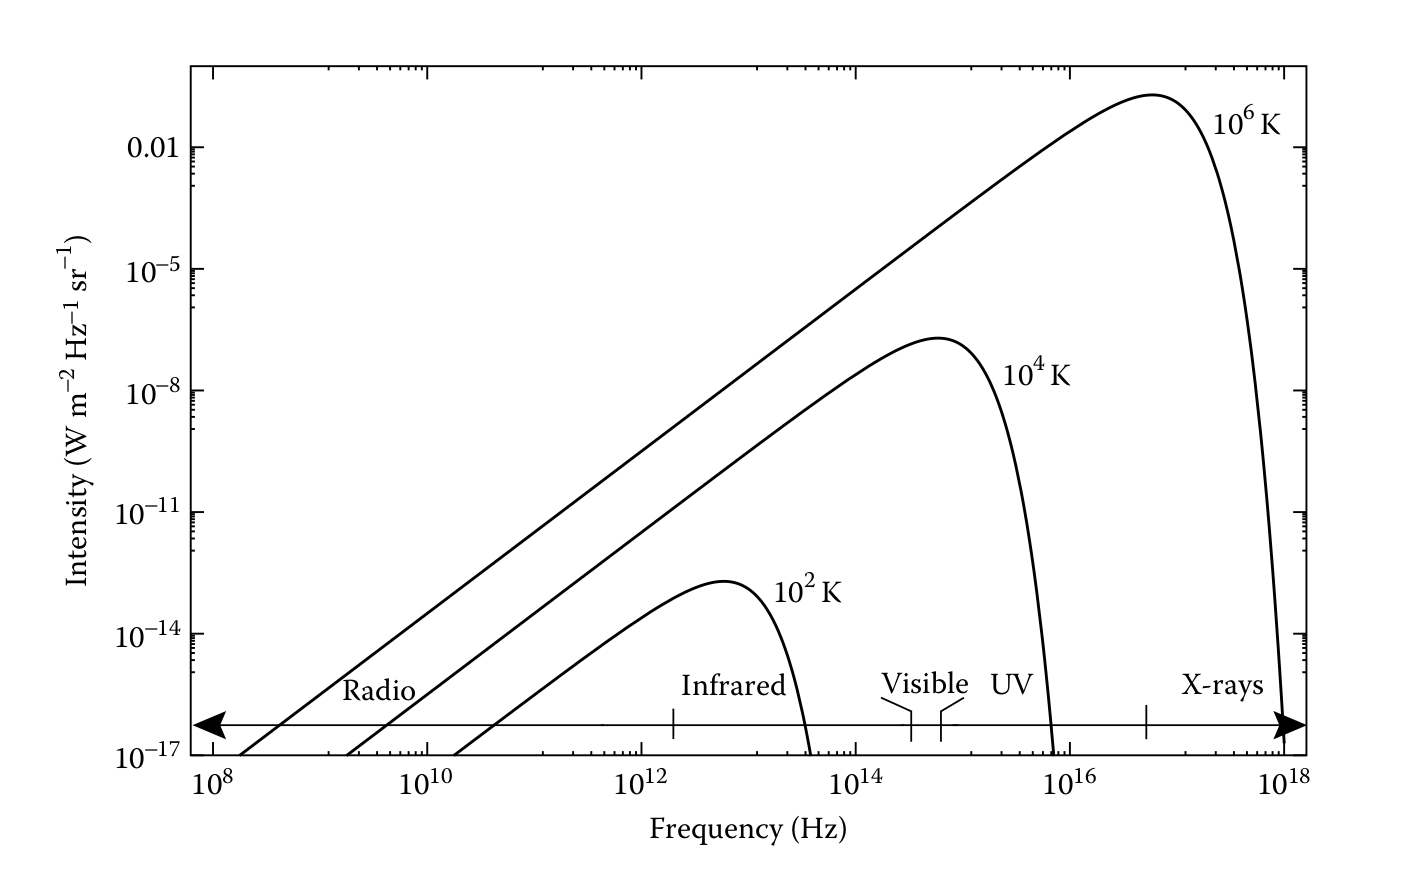
\includegraphics[width=0.7\textwidth]{Images/B_nu_plot.png}
	\caption{Log-log plot of $B_{\nu}(T)$ versus $\nu$ for three different temperatures.}
	\label{fig:planckfunctionnu}
\end{figure}

\begin{figure}[H]
	\centering
	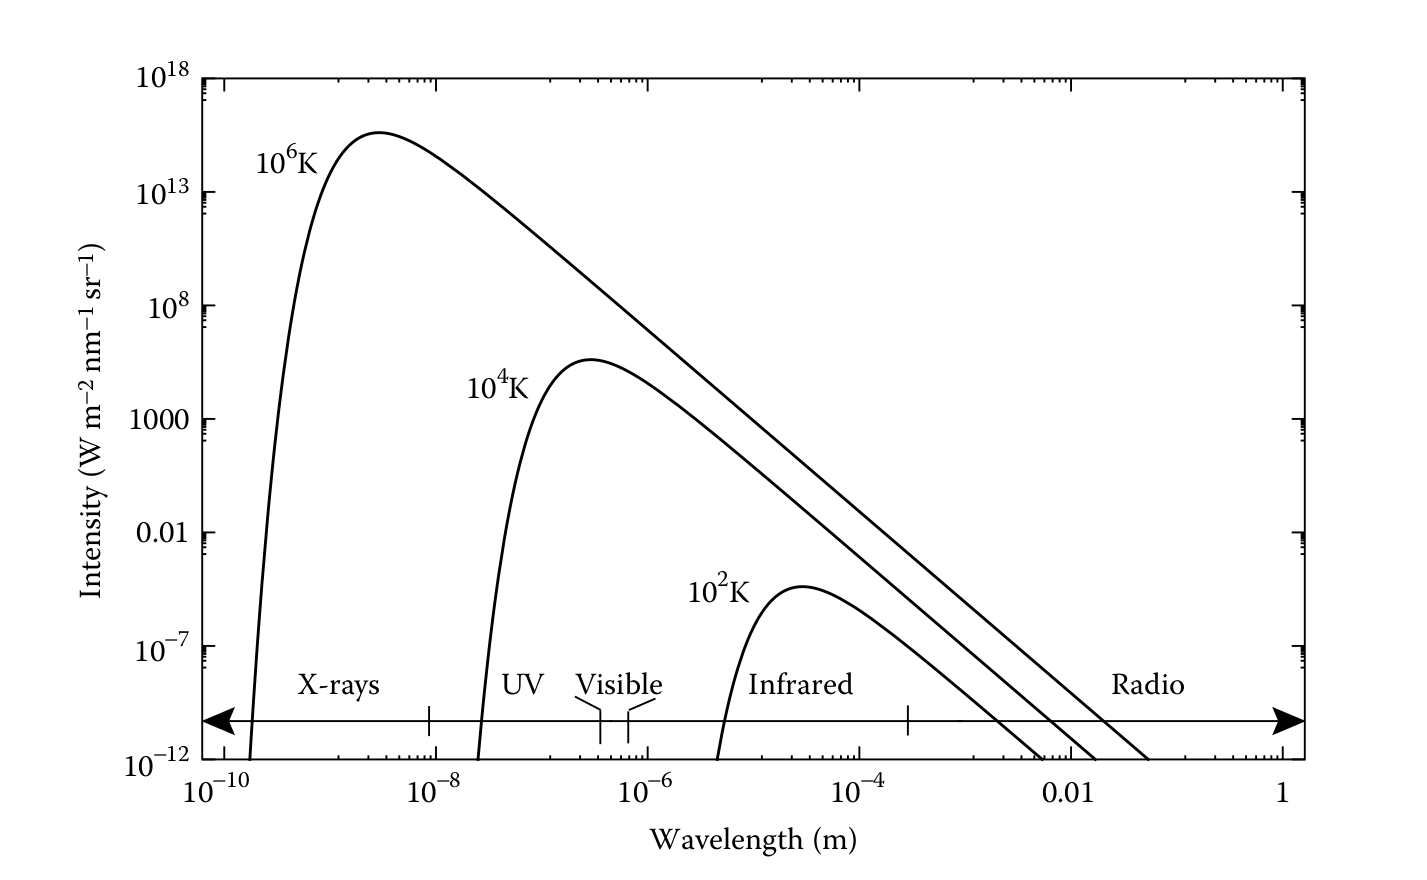
\includegraphics[width=0.7\textwidth]{Images/B_lambda_plot.png}
	\caption{Log-log plot of $B_{\lambda}(T)$ versus $\lambda$ for three different temperatures.}
	\label{fig:planckfunctionlambda}
\end{figure}

The total flux of radiation (\(\text{W m}^{-2}\)) emitted by the body can be obtained by integration of the Planck function over frequency and solid angle. The result shows that the total flux is given by

\begin{equation}
	F = \sigma T^4
	\label{eq:stefanboltzmannlaw}
\end{equation}

where \(\sigma\) is the Stefan-Boltzmann constant. This is an expression of the Stefan–Boltzmann law. Another very useful result can be obtained by finding the frequency of the peak intensity of the Planck function. This frequency, \(\nu_\text{max}\), is proportional to the body’s temperature and is given by Wien’s displacement law, which states

\[
\nu_\text{max} = 2.82 \frac{kT}{h}
\]

Finally, it is also useful to calculate the brightness temperature of a source whose intensity is \(I_\nu\). This brightness temperature, \(T_B\), is the temperature at which a blackbody would emit with an intensity equal to \(I_\nu\). That is, it is found by solving for \(T\) in the expression

\[
I_\nu = B_\nu(T)
\]

As mentioned above, radio astronomers typically express the Planck function using frequency (\(\nu\)) rather than wavelength (\(\lambda\)). Radio astronomers also express the Planck function in a modified form using temperature units. The brightness temperature of a source whose specific intensity is \(I_\nu\) is defined as the temperature of a blackbody that would emit the same specific intensity, \(T_B\), at the frequency \(\nu\). The Planck function in the Rayleigh–Jeans approximation can be expressed as

\[
B_\nu(T) \approx \frac{2\nu^2 kT}{c^2}
\]

The brightness temperature of a source with intensity \(I_\nu\) is then

\[
T_B \approx \frac{I_\nu c^2}{2k\nu^2}
\]

\section{Rayleigh-Jeans Approximation}

At most radio wavelengths, the Planck function can be approximated by a much simpler expression, which makes for much easier math when using it. At most radio wavelengths, the frequency, $\nu$, is so small that $\frac{h \nu}{k T} \ll 1$ for any reasonable temperature. The exponential in the denominator of the Planck function then can be approximated by a Taylor series expansion, yielding

\begin{equation}
\frac{1}{e^{h\nu/kT} - 1} \approx \frac{kT}{h\nu} \quad \text{for} \quad \frac{h\nu}{kT} \ll 1
\label{eq:taylor}
\end{equation}

and so,

\begin{equation}
B_\nu (T) \approx \frac{2h\nu^3}{c^2} \cdot \frac{kT}{h\nu} = \frac{2k\nu^2}{c^2} T
\label{eq:rayleigh_jeans_freq}
\end{equation}

or

\begin{equation}
B_\nu (T) \approx \frac{2kT}{\lambda^2}
\label{eq:rayleigh_jeans_wave}
\end{equation}

Note how simple this expression is in comparison to the Planck function (Equation~\eqref{eq:planckfunctionfrequency}). This expression is very useful, provided you are in the realm where $\frac{h \nu}{k T} \ll 1$. This expression is known as the Rayleigh--Jeans approximation, often referred to as the Rayleigh--Jeans law.

\clearpage

\section{Brightness Temperature}

Brightness temperature (\( T_B \)) is an important parameter in radio astronomy, providing a convenient way to describe the intensity of radiation using the Rayleigh–Jeans approximation. This approximation shows that at radio wavelengths, the intensity (\( B_\nu(T) \)) of radiation emitted by a blackbody is directly proportional to its temperature (\( T \)), i.e., \( B_\nu(T) \propto T \). \\

At radio wavelengths, intensity and temperature of blackbody sources can be used interchangeably and are linearly related by \( \frac{2k}{\lambda^2} \). In the Rayleigh–Jeans approximation, the brightness temperature is defined as:

\[
T_B = \frac{\lambda^2}{2k} I_\nu
\]

\( T_B \) is a property of the radiation, not the emitting object. For an opaque thermal source, \( T_B \) directly represents the object's temperature. However, it only equals the source's temperature when the source is both thermal and opaque. \\

At higher frequencies or lower temperatures, where \( h\nu \) is not much smaller than \( kT \), the Rayleigh–Jeans approximation is insufficient. In such cases, the full Planck function must be used:

\[
I_\nu = B_\nu(T_B) = \frac{2h\nu^3}{c^2} \left( \frac{1}{e^{h\nu/kT_B} - 1} \right)
\]

Brightness temperature measures intensity and equals the temperature of an opaque thermal source at low frequencies. For non-thermal radiation (e.g., synchrotron radiation), \( T_B \) is not related to the source temperature but still describes radiation intensity. \\

Temperature descriptions for intensity or radiation power also appear in other contexts, such as antenna temperature, noise temperature, receiver temperature, and system temperature, representing power per unit frequency in radio telescope observations. \\

\clearpage

\section{Coherent Radiation}

The radio-wavelength radiation emitted by an individual electron is undetectable by any radio telescope; what we detect is the sum of emissions from many electrons. There are two main ways electromagnetic waves from different electrons can combine, which significantly affects how we treat the radiation mathematically and its physical properties.

Imagine a single electron oscillating at a fixed frequency, emitting electromagnetic waves at a single wavelength. If multiple wave chains, all in phase, join this initial chain, they amplify the initial wave constructively, resulting in coherent radiation. This is similar to what happens in a laser.

In contrast, incoherent radiation occurs when many unrelated electrons emit radiation independently, as in an incandescent light bulb. The resulting waves have random phases and cannot be modeled by a single chain of sine waves.

\begin{figure}[H]
	\centering
	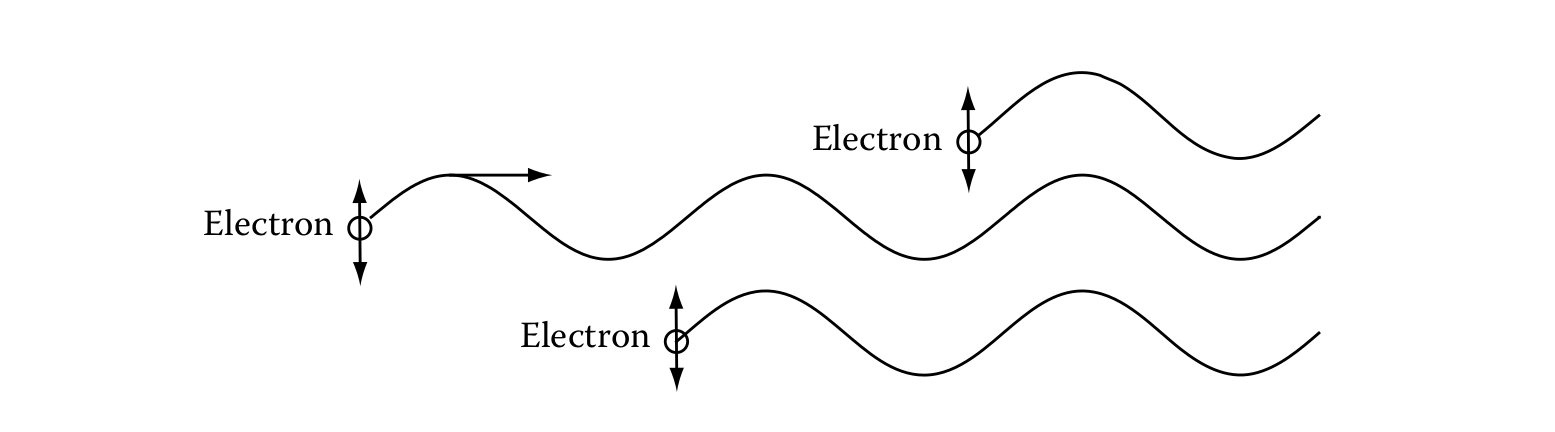
\includegraphics[width=0.5\textwidth]{Images/coherent_radiation.png}
	\caption{Creation of Coherent Radiation.}
	\label{fig:coherent_radiation}
\end{figure}

Mathematically, coherence of radiation means that at any location in space and time, the radiation has a specific phase. To understand coherence, consider two electromagnetic wave chains with identical frequencies and directions, but with a phase difference. Representing the waves as cosines:

\[
E_1 = E_0 \cos(\omega t)
\]
\[
E_2 = E_0 \cos(\omega t + \Delta \phi)
\]

Their sum is:

\[
E_1 + E_2 = E_0 \cos(\omega t) + E_0 \cos(\omega t + \Delta \phi)
\]

The intensity (\( I \)) is proportional to the square of the electric field, averaged over time. The intensity of each wave chain is:

\[
I_1 = I_2 = \alpha E_0^2 / 2
\]

The total intensity is:

\[
I_{\text{total}} = \alpha (E_1 + E_2)^2 = \alpha E_0^2 \left[1 + \cos(\Delta \phi)\right]
\]

When waves are in phase (\( \Delta \phi = 0 \)), \( \cos(\Delta \phi) = 1 \), and the total intensity is four times that of an individual wave. For incoherent light, the interference term averages to zero, resulting in the total intensity being the sum of individual intensities.

In summary, incoherent light results in a total intensity equal to the sum of component intensities, while coherent light's intensity grows as the square of the sum of the component intensities. Despite the differing intensities, the total energies remain conserved, with coherent light having a higher intensity over a smaller wavelength range and a narrower beam.


\clearpage

\section{Interference of Light}

\clearpage

\section{Polarization of Light}

\clearpage

\section{Cosmic Microwave Background}

The Cosmic Microwave Background (CMB) is the thermal radiation left over from the Big Bang. It is a faint glow of light that fills the universe in all directions. The CMB is a critical piece of evidence supporting the Big Bang theory and provides a wealth of information about the universe's early history. \\

The CMB was first discovered by Arno Penzias and Robert Wilson in 1965. They were conducting radio astronomy experiments using a horn antenna at Bell Labs in New Jersey when they detected an unexpected background noise. After ruling out all possible sources of interference, they realized they had discovered the CMB. \\

We use data from COBE~\cite{1990ApJ...354L..37M} Satellite to fit the Planck function to the CMB data. We fit the Planck function to the data and determine the temperature of the CMB. The Planck function is already defined in section~\ref{sec:blackbodyradiation}.

\begin{figure}[H]
	\centering
	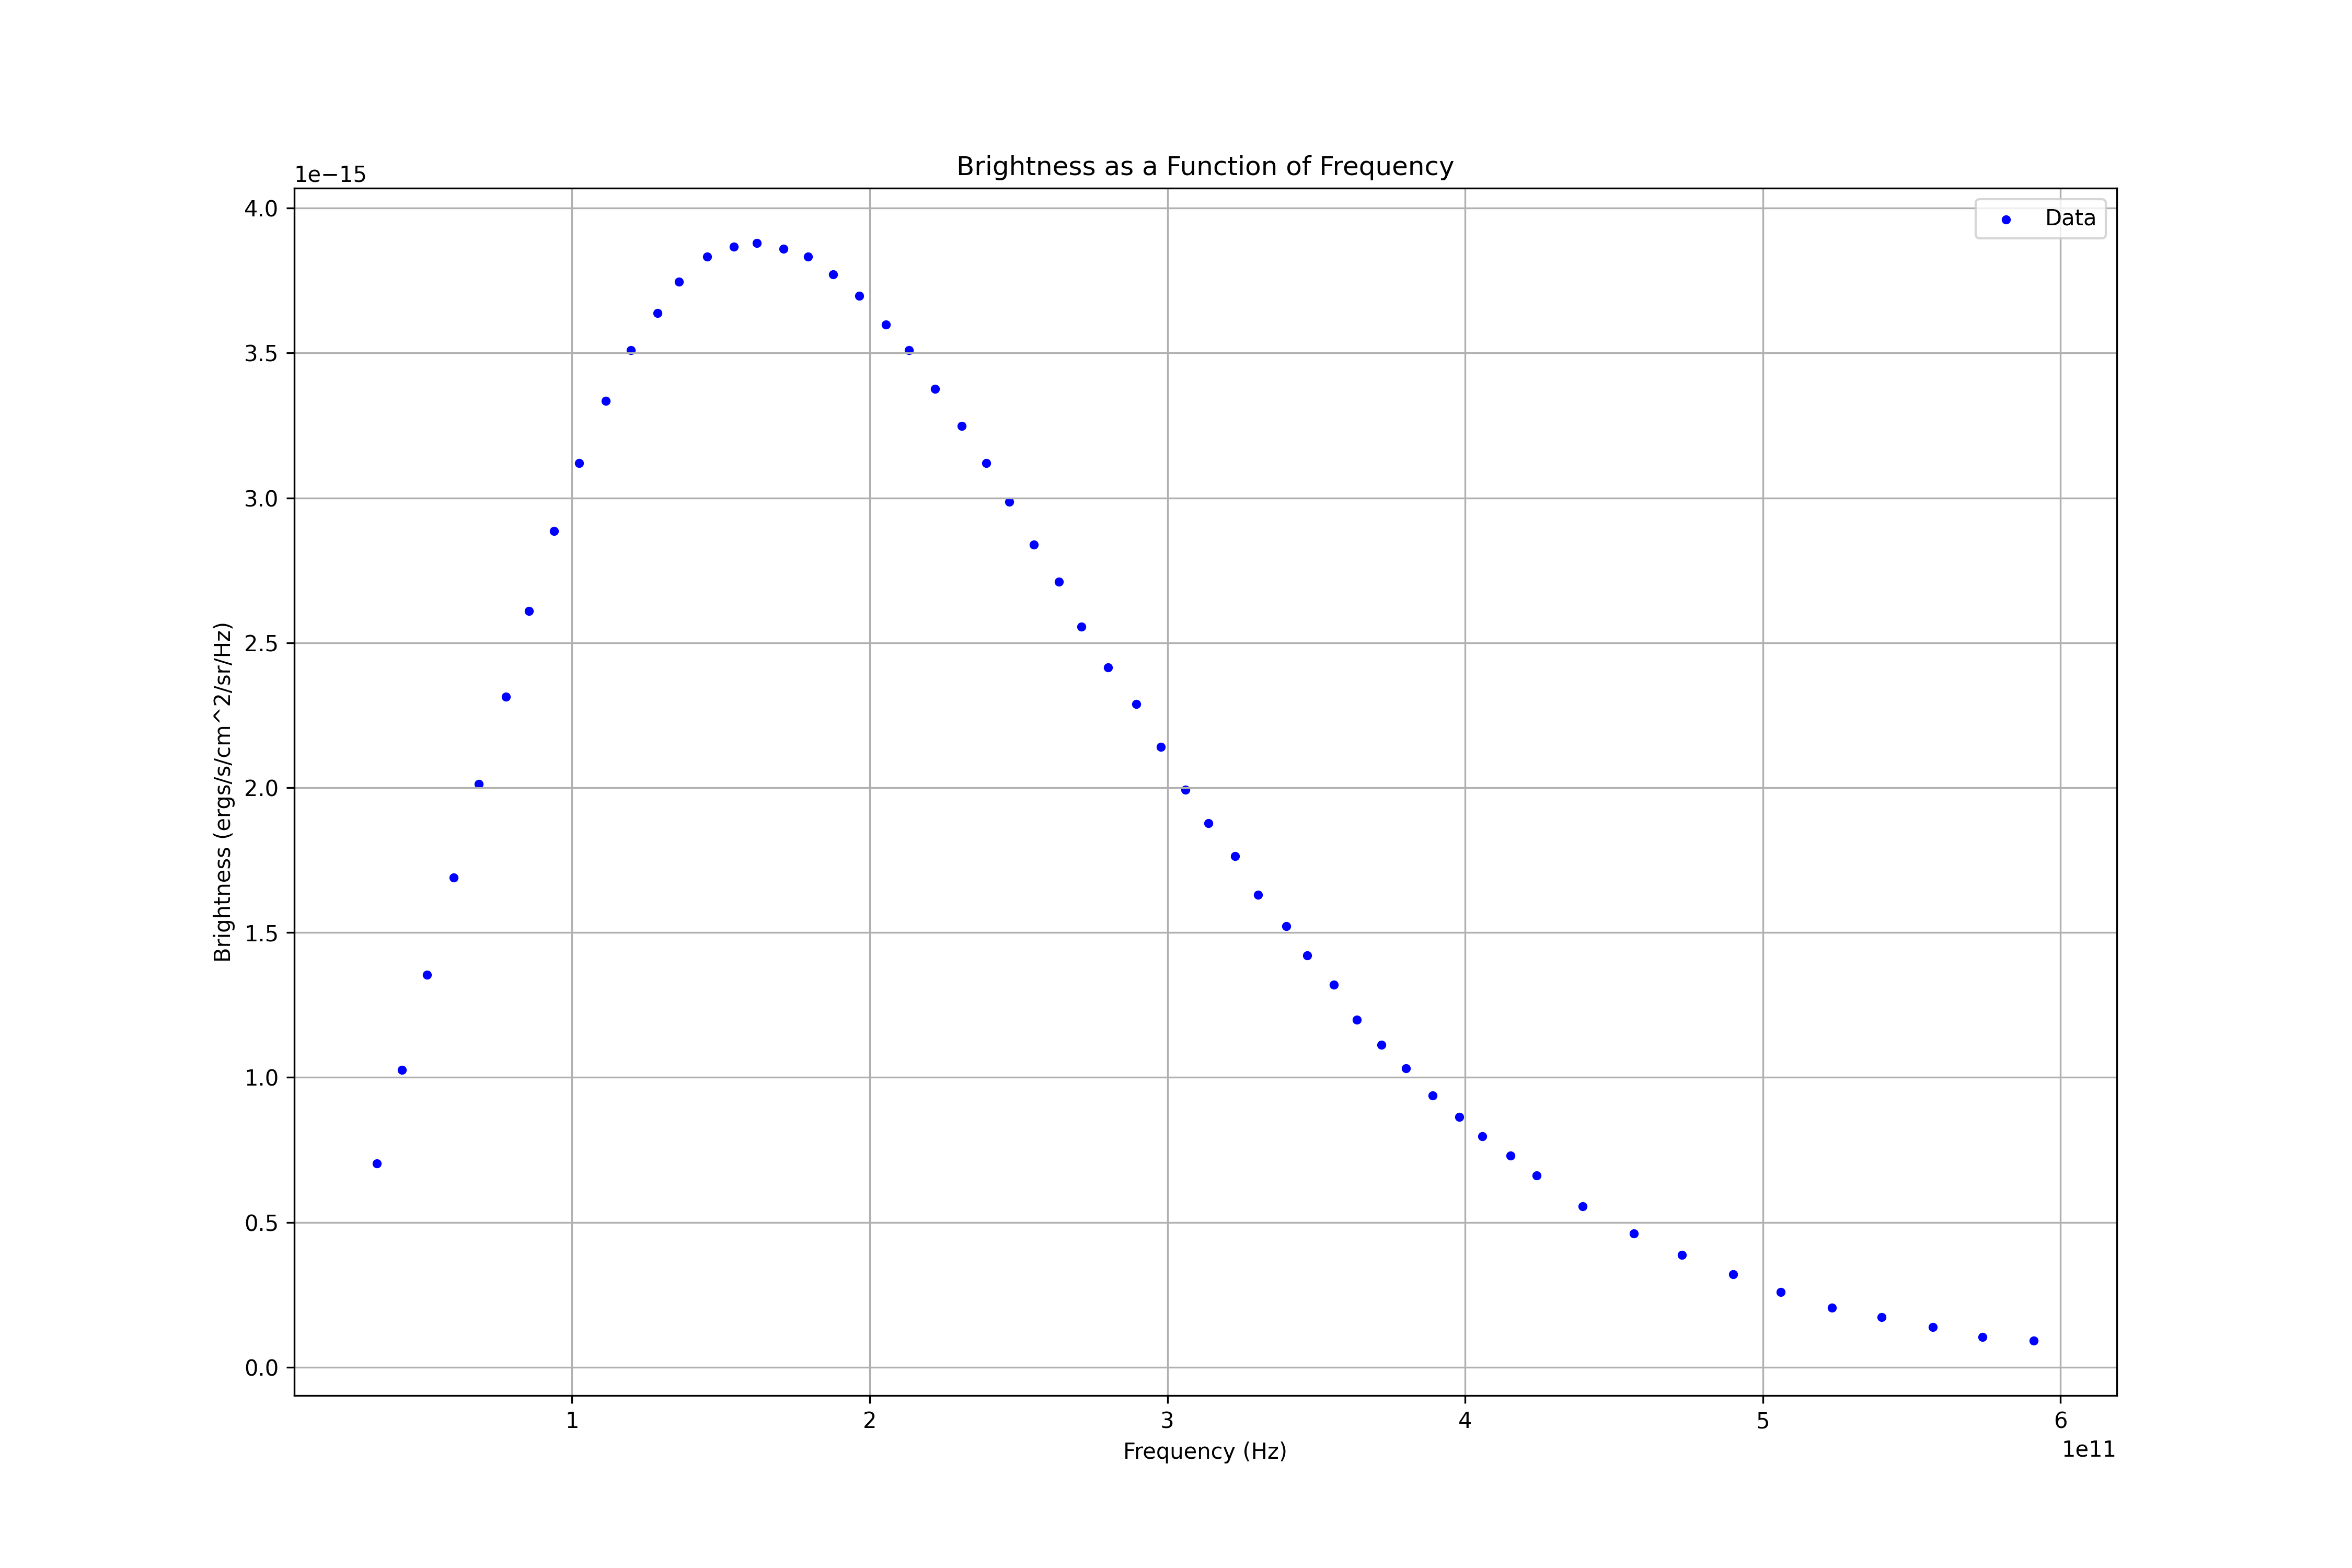
\includegraphics[width=\textwidth]{Images/COBE_CMB_data.png}
	\caption{Plotted CMB Data}
	\label{fig:cmb_fit}
\end{figure}

Using the blackbody function, we get the optimized CMB temperature to be \textbf{2.738305 K.}

\clearpage

\section{Hydrogen 21cm Line \& Galaxy Rotation Curve}

The Hydrogen $21$cm line is a very important spectral line important in radio astronomy as it is used to study the distribution of neutral atomic hydrogen in the interstellar medium. The $21$cm line is a hyperfine transition of the hydrogen atom, which occurs due to the spin-flip transition of the electron in the hydrogen atom. This line is important in studying the dynamics of galaxies and the distribution of hydrogen in the Universe. \\

The $21$cm line is used to study the rotation curve of galaxies. The rotation curve of a galaxy is a plot of the orbital velocity of the stars and gas in the galaxy as a function of the distance from the center of the galaxy. The rotation curve of a galaxy is important in studying the mass distribution of the galaxy. The rotation curve of a galaxy is used to study the dark matter distribution in the galaxy. \\

To obtain the galaxy rotation curve, we will use synthetic spectra available for different spectrums of different distance intervals within that is a Hydrogen 21 cm line at a Doppler velocity. We fit for the Doppler velocity of the 21 cm line for each distance. To do so, we fit a gaussian to the spectral line and determine the central frequency. We Use the displacement from the expected value to find the velocity. Once all lines are done, plot the velocities as a function of distance from the centre of our galaxy.

\begin{figure}[H]
	\centering
	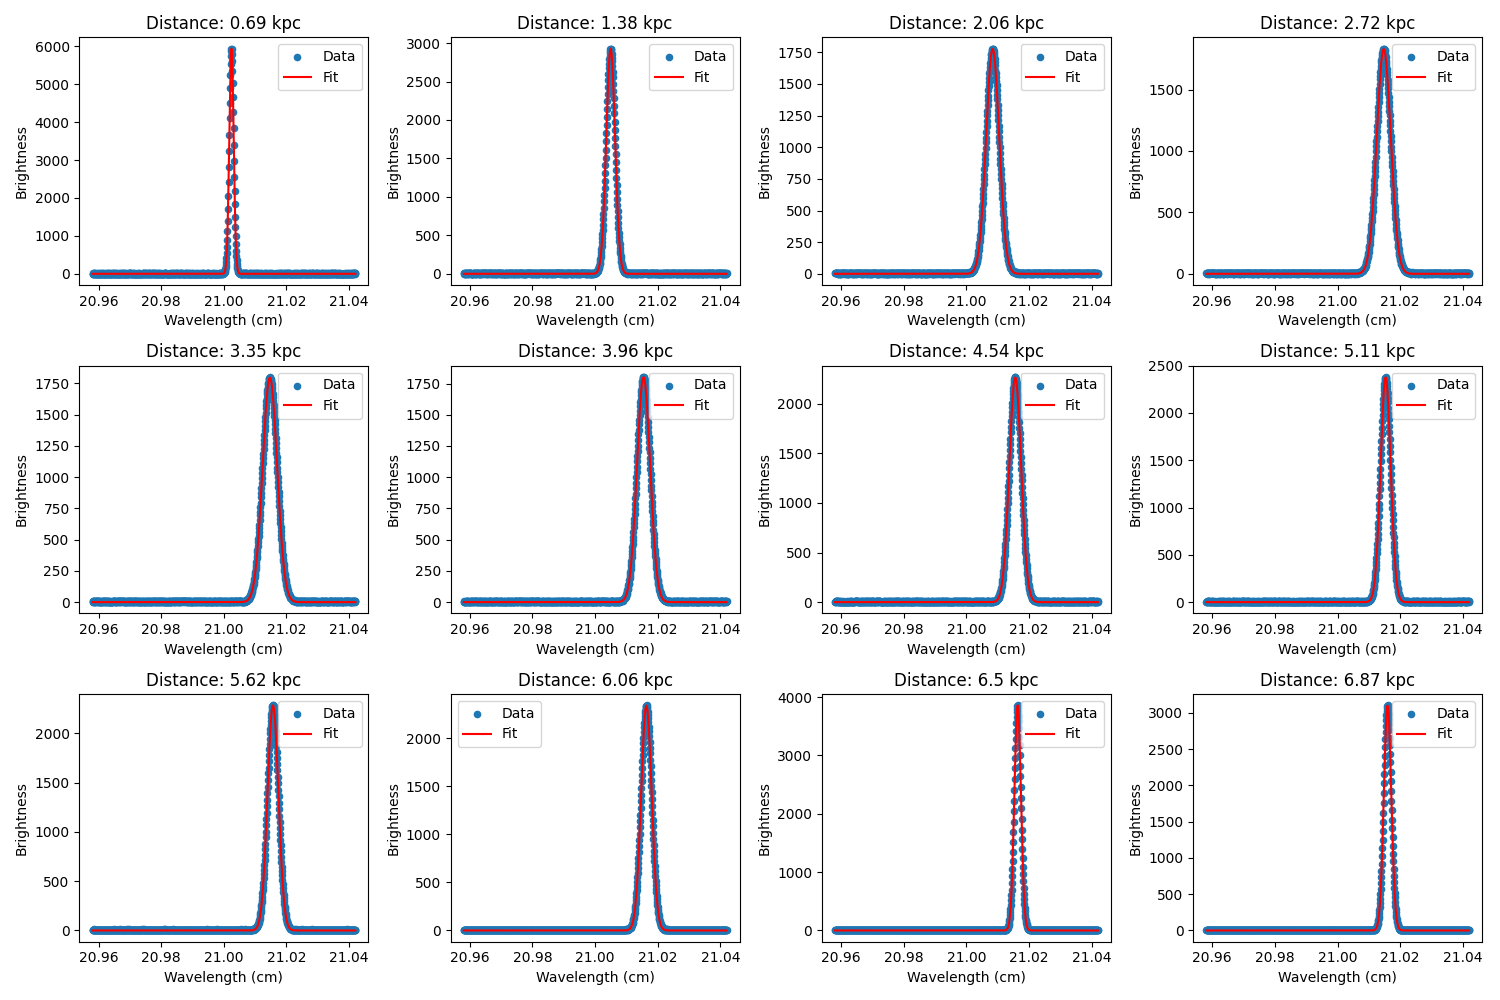
\includegraphics[width=\textwidth]{Images/12_files.png}
	\caption{Plots for each distance}
	\label{fig:12_files}
\end{figure}

Using the data obtained from the Gaussian fits, we can plot the velocities as a function of distance from the centre of the galaxy. 

\begin{figure}[H]
	\centering
	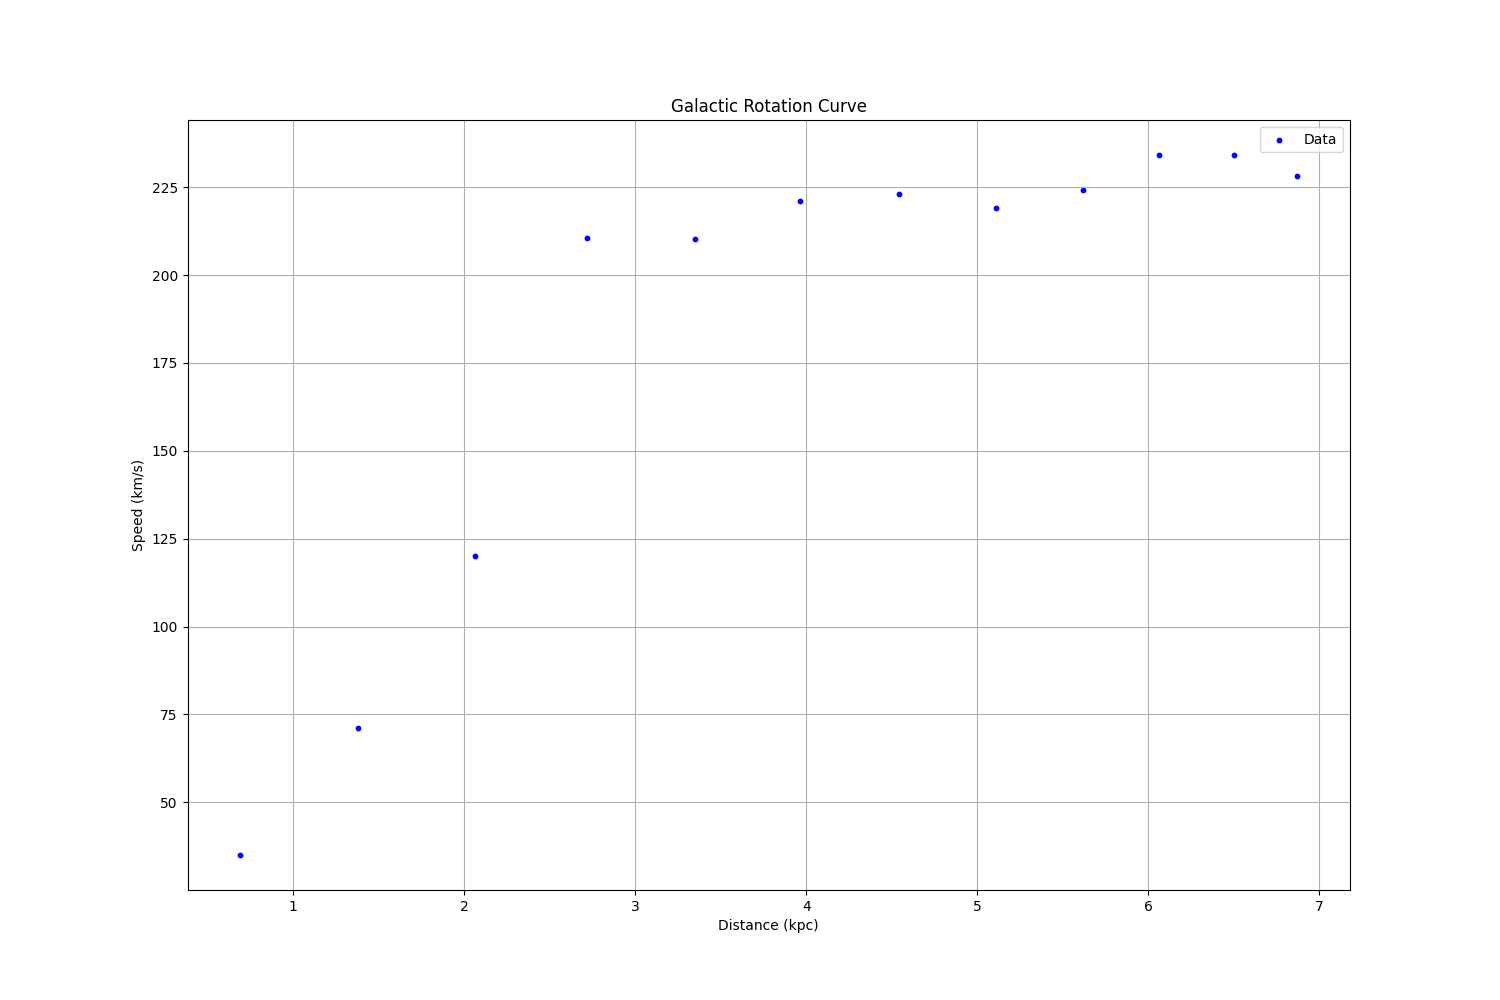
\includegraphics[width=\textwidth]{Images/galaxy_rotation_curve.png}
	\caption{Galaxy Rotation Curve}
	\label{fig:galaxy_rotation_curve}
\end{figure}
\chapter{Radio Telescopes}

\section{Reflectors, Antennas and Feeds}

Radio telescopes are sophisticated instruments designed to detect and analyze radio waves from astronomical sources. The core components of a radio telescope include the reflector, the antenna, and the feed. These elements work together to capture, focus, and convert radio frequency signals into a form that can be analyzed by astronomers. This section delves into the specifics of these components and their roles in the functionality of radio telescopes.

\subsection{Reflectors}

The reflector is a crucial part of a radio telescope, serving the purpose of collecting and focusing incoming radio waves onto the antenna. The most common type of reflector used in radio telescopes is the parabolic reflector. This shape ensures that radio waves parallel to the axis of the dish are reflected to a single focal point. The main features of parabolic reflectors include:

\begin{itemize}
    \item \textbf{Shape:} A paraboloid of revolution, ensuring that all incoming parallel rays are focused at the focal point.
    \item \textbf{Surface Accuracy:} The precision of the reflector surface must be within a fraction of the wavelength of the observed radio waves to avoid significant signal loss.
    \item \textbf{Size:} Reflector sizes vary, with larger dishes collecting more signal and thus allowing for the detection of weaker sources.
\end{itemize}

\subsection{Antennas}

The antenna in a radio telescope system is responsible for receiving the radio waves focused by the reflector. Several types of antennas can be used, each with its unique characteristics:

\begin{itemize}
    \item \textbf{Dipole Antennas:} Simple and effective for a range of frequencies, often used in conjunction with other elements to form more complex arrays.
    \item \textbf{Horn Antennas:} Common in microwave frequencies, providing a directional response and often used in combination with parabolic reflectors.
    \item \textbf{Array Antennas:} Consist of multiple antenna elements arranged to work together, increasing sensitivity and resolution.
\end{itemize}

Antennas convert the focused radio waves into electrical signals that can then be processed and analyzed.

\subsection{Feeds}

The feed is the interface between the reflector and the antenna. It collects the focused radio waves from the reflector and directs them to the antenna. There are different types of feeds used in radio telescopes:

\begin{itemize}
    \item \textbf{Prime Focus Feed:} Positioned at the focal point of the reflector, it directly collects the focused radio waves.
    \item \textbf{Cassegrain Feed:} Uses a secondary reflector to redirect the radio waves to a focus near the primary reflector's vertex, often allowing for more convenient placement of the receiving equipment.
    \item \textbf{Gregorian Feed:} Similar to the Cassegrain but with a concave secondary reflector, used to correct certain optical aberrations.
\end{itemize}

The choice of feed depends on factors such as the desired frequency range, the size of the reflector, and the specific scientific goals of the telescope.

In conclusion, the efficiency and effectiveness of a radio telescope depend on the precise interplay between its reflectors, antennas, and feeds. Each component must be carefully designed and optimized to ensure the maximum capture and accurate conversion of radio frequency signals from distant astronomical sources. 

\section{Heterodyne Receivers}

The purposes of the radio telescope receiver are to define the frequency range, or passband, over which the received power will be collected, and to produce a signal proportional to the collected power that can be recorded. The components that make up a receiver are often divided between two separate sections referred to as the front-end receiver and the back-end receiver.

\begin{figure}[H]
	\centering
	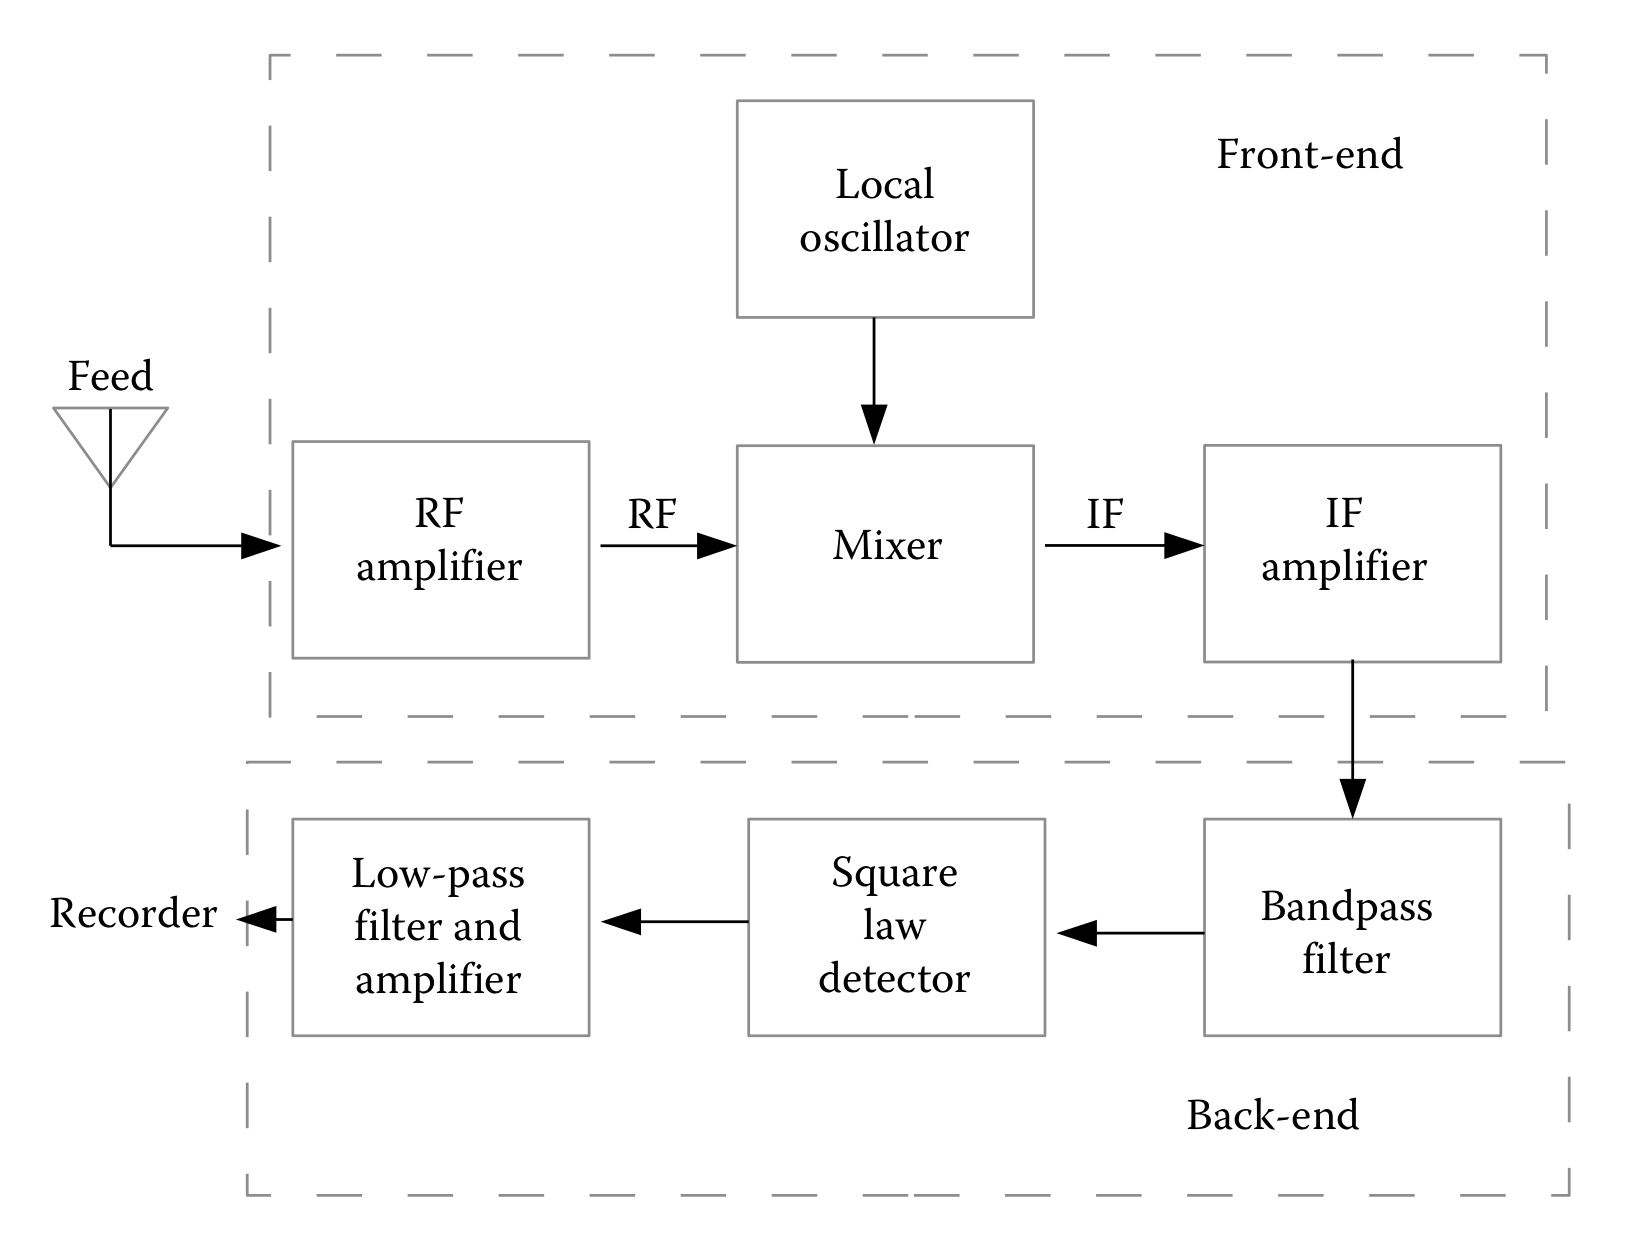
\includegraphics[width=0.8\textwidth]{Images/telescope_components.png}
	\caption{Components of a radio telescope receiver.}
	\label{fig:telescope_components}
\end{figure}

\subsection{Transmission Lines}

There are several types of transmission lines, such as waveguides and coaxial cables, used in radio telescope receivers. These transmission lines carry the electromagnetic waves from the feed to the detector. Waveguides are suitable for higher frequencies, while coaxial cables are more flexible but have higher signal loss.

\begin{figure}[H]
    \centering
    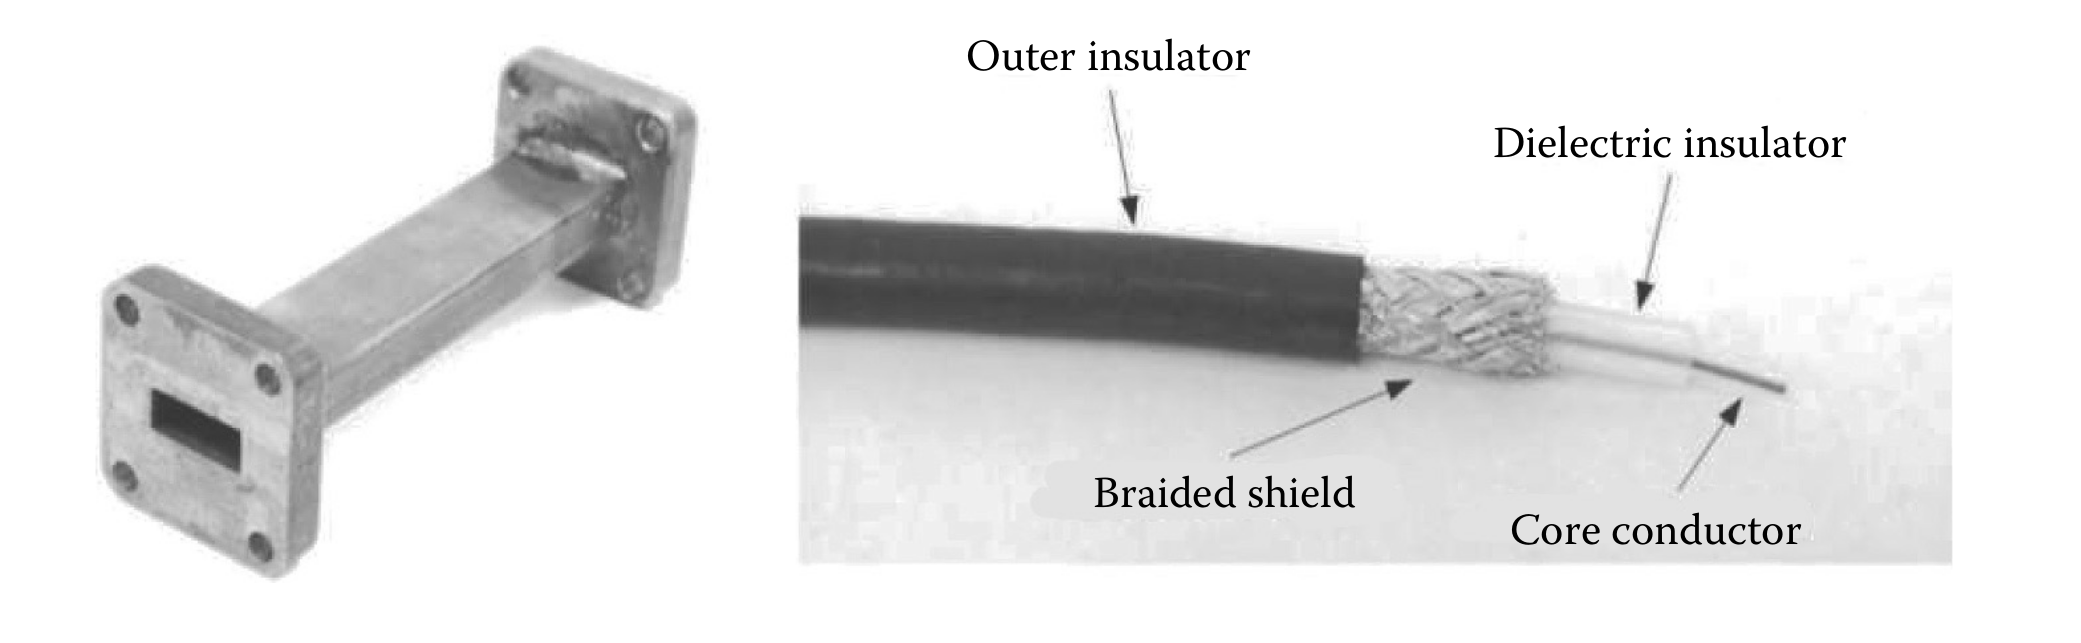
\includegraphics[width=0.8\textwidth]{Images/waveguide_coaxial.png}
    \caption{Examples of transmission lines: rectangular waveguide (left) and coaxial cable (right).}
    \label{fig:transmission_lines}
\end{figure}

\subsection{Front-End Receiver Components}

The front-end receiver components process the incoming radio frequency (RF) signals. Key components include:

\begin{itemize}
    \item \textbf{RF Amplifier:} Increases the amplitude of the RF signal.
    \item \textbf{Local Oscillator (LO):} Generates a signal used in the mixing process.
    \item \textbf{Mixer:} Combines the RF and LO signals to produce an intermediate frequency (IF) signal.
    \item \textbf{IF Amplifier:} Amplifies the IF signal for further processing.
    \item \textbf{Bandpass Filter:} Selects a narrow range of frequencies to pass to the back-end.
\end{itemize}

\subsection{Back-End Receiver Components}

The back-end receiver processes the IF signal received from the front-end. Components include:

\begin{itemize}
    \item \textbf{Bandpass Filter:} Defines the range of frequencies to detect.
    \item \textbf{Square-Law Detector:} Measures the power of the IF signal.
    \item \textbf{Low-Pass Filter:} Removes high-frequency components from the detector output.
    \item \textbf{DC Amplifier:} Amplifies the signal for digital conversion and recording.
\end{itemize}

\subsection{High-Frequency Heterodyne Receivers}

At frequencies above 300 GHz, special high-frequency heterodyne receivers are used. These receivers mix the RF signal with the IF first, then amplify the IF signal. They require low-noise components and are often based on superconducting materials.
\chapter{Imaging Radio Sources using CASA}

\section{Introduction}

CASA, or Common Astronomy Software Applications, is a suite of tools developed by the National Radio Astronomy Observatory (NRAO) to process radio interferometric data. It is a powerful tool that can be used to calibrate, image and analyze radio interferometric data. In this section, we will discuss how to use CASA to image radio sources.

% Inferometry

\subsection{Interferometry}

Interferometry is a technique used in radio astronomy to combine signals from multiple telescopes to form a single image. The basic idea behind interferometry is to use the interference pattern created by the combination of signals from multiple telescopes to reconstruct an image of the sky. The resolution of an interferometer is determined by the distance between the telescopes, with larger distances resulting in higher resolution images.

% CASA

\subsection{CASA}

CASA is a software package that is specifically designed to process radio interferometric data. It provides a wide range of tools for calibrating, imaging and analyzing radio interferometric data. CASA is widely used in the radio astronomy community and is the standard software package used for processing data from radio interferometers such as the Atacama Large Millimeter Array (ALMA) and the Very Large Array (VLA).

\clearpage

\section{TW Hydra}

In this section, we will use CASA to image the radio source TW Hydra. TW Hydra is a young star located in the constellation Hydra, approximately 176 light years from Earth. It is a popular target for radio observations due to its proximity and young age.

\subsection{`plotms' command}

The `plotms' command in CASA is used for UV data visualization. It can be used to plot visibility data from a measurement set and provides a range of options for customizing the plot. The `plotms' command is a useful tool for visualizing the visibility data and identifying any issues with the data.

\lstdefinestyle{casa-python}{
       language=Python,
       keywordstyle=\color{blue}\bfseries,
       commentstyle=\color{green},
       stringstyle=\color{red},
       numberstyle=\color[rgb]{0.205, 0.142, 0.73},
       basicstyle=\ttfamily\footnotesize,
       breaklines=true,
       frame=single,
       numbers=left,
       numberstyle=\tiny\color{gray},
       stepnumber=1,
       tabsize=4,
       showspaces=false,
       showstringspaces=false,
       showtabs=false,
       captionpos=b,
       morekeywords={vis, xaxis, yaxis, axis, avgchannel, avgspw, avgtime, avgscan, coloraxis, showgui, imagename, field, spw, specmode, deconvolver, gridder, imsize, cell, weighting, threshold, niter, interactive, width, outputvis, robust, datacolumn, mask}, % Add CASA-specific keywords if needed
       upquote=true,
}

\vspace{15mm}

\begin{lstlisting}[style=casa-python]
plotms(vis='sis14_twhya_calibrated_flagged.ms', 
       xaxis='u', 
       yaxis='v', 
       avgchannel='10000', 
       avgspw=False, 
       avgtime='1e9', 
       avgscan=False, 
       coloraxis="field", 
       showgui=True)
\end{lstlisting}

\begin{figure}[H]
	\centering
	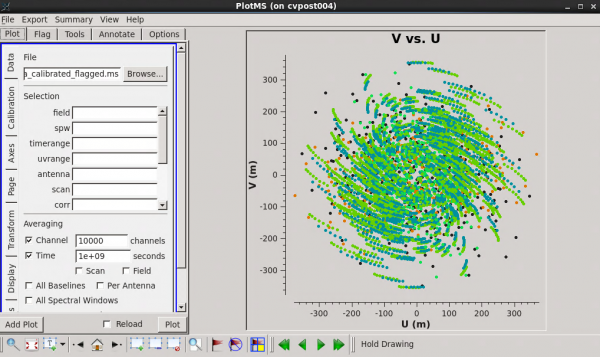
\includegraphics[width=0.8\textwidth]{Images/uv.png}
	\caption{Plot of visibility data for TW Hydra using the `plotms' command in CASA.}
\end{figure}

\clearpage

\subsection{`tclean' command}

The `tclean' command in CASA is used to image the radio source using the visibility data from a measurement set. The `tclean' command uses a deconvolution algorithm to reconstruct the image of the sky from the visibility data. The `tclean' command can be used to create high resolution images of radio sources.

\vspace{15mm}

\begin{lstlisting}[style=casa-python]
tclean(vis='sis14_twhya_calibrated_flagged.ms',
   imagename='phase_cal',
   field='3',
   spw='',
   specmode='mfs',
   deconvolver='hogbom',
   gridder='standard',
   imsize=[128,128],
   cell=['0.1arcsec'],
   weighting='briggs',
   threshold='0mJy',
   niter=5000,
   interactive=True)
\end{lstlisting}

\begin{figure}[H]
	\centering
	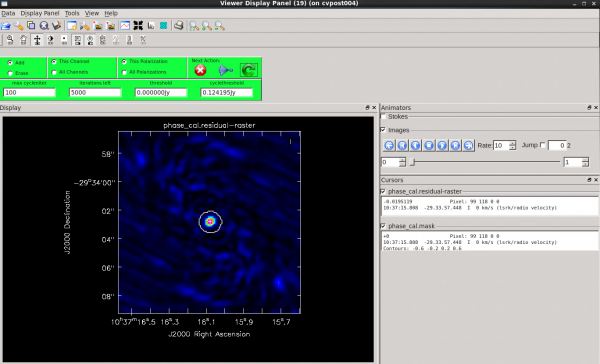
\includegraphics[width=0.8\textwidth]{Images/tclean.png}
	\caption{The tclean GUI showing the clean mask (white oval) circling the emission region.}
\end{figure}

\clearpage

\subsubsection{Using Briggs Weighing}

\begin{lstlisting}[style=casa-python]
tclean(vis='sis14_twhya_calibrated_flagged.ms',
       imagename='phase_cal_robust',
       field='3',
       spw='',
       specmode='mfs',
       gridder='standard',
       deconvolver='hogbom',
       imsize=[128,128],
       cell=['0.1arcsec'],
       weighting='briggs',
       robust=-1.0,
       threshold='0mJy',
       niter=5000,
       interactive=True)
\end{lstlisting}

\begin{figure}[H]
	\centering
	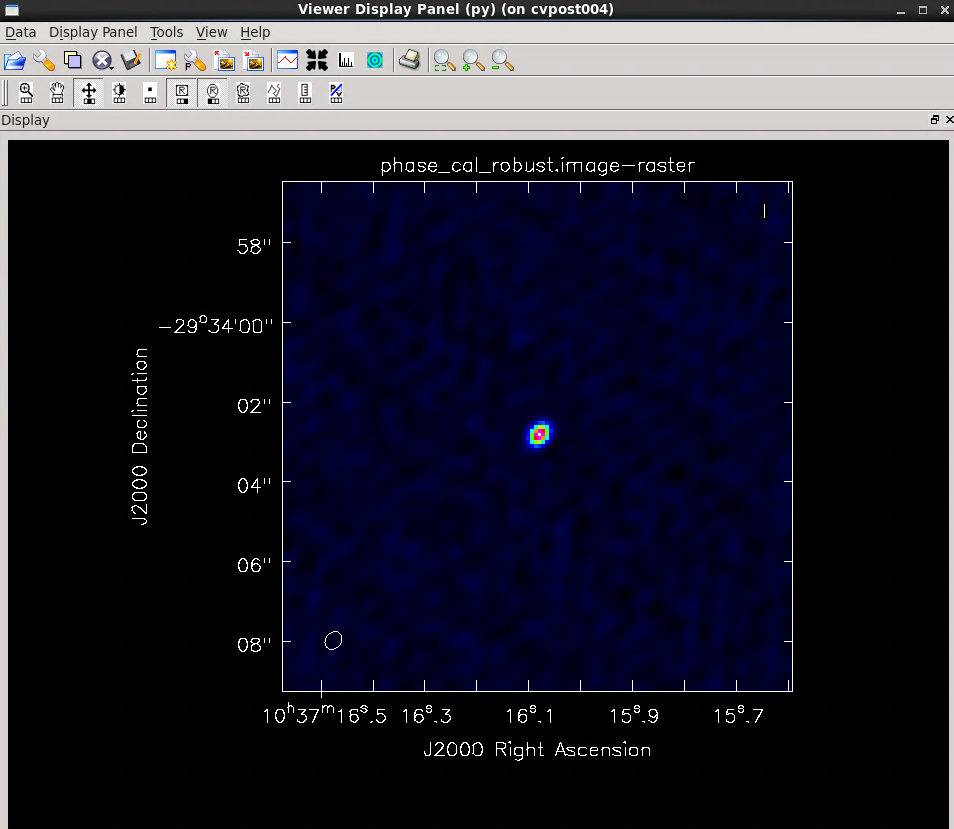
\includegraphics[width=0.8\textwidth]{Images/tclean-robust.png}
	\caption{Viewer image of the phase calibrator after tclean with briggs weighting.}
\end{figure}

\clearpage

\subsubsection{Increasing the Pixel size}

\begin{lstlisting}[style=casa-python]
tclean(vis='sis14_twhya_uncalibrated.ms',
       imagename='phase_cal_uncalibrated',
       field='3',
       spw='',
       specmode='mfs',
       gridder='standard',
       deconvolver='hogbom',
       imsize=[128,128],
       cell=['0.1arcsec'],
       weighting='natural',
       threshold='0mJy',
       niter=5000,
       interactive=True)
\end{lstlisting}

\begin{figure}[H]
       \centering
       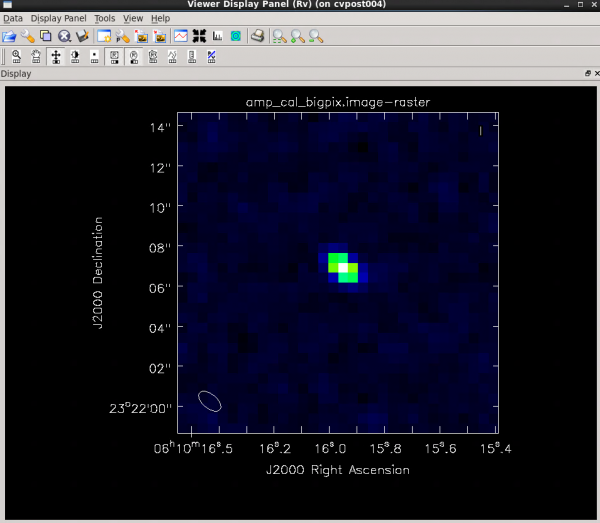
\includegraphics[width=0.8\textwidth]{Images/large-pixel-size.png}
       \caption{Viewer image of the amplitude calibrator after tclean with a large pixel size.}
\end{figure}

\clearpage

\subsubsection{Effects of Uncaliberated Data}

\begin{lstlisting}[style=casa-python]
tclean(vis='sis14_twhya_uncalibrated.ms',
       imagename='phase_cal_uncalibrated',
       field='3',
       spw='',
       specmode='mfs',
       gridder='standard',
       deconvolver='hogbom',
       imsize=[128,128],
       cell=['0.1arcsec'],
       weighting='natural',
       threshold='0mJy',
       niter=5000,
       interactive=True)
\end{lstlisting}

\begin{figure}[H]
       \centering
       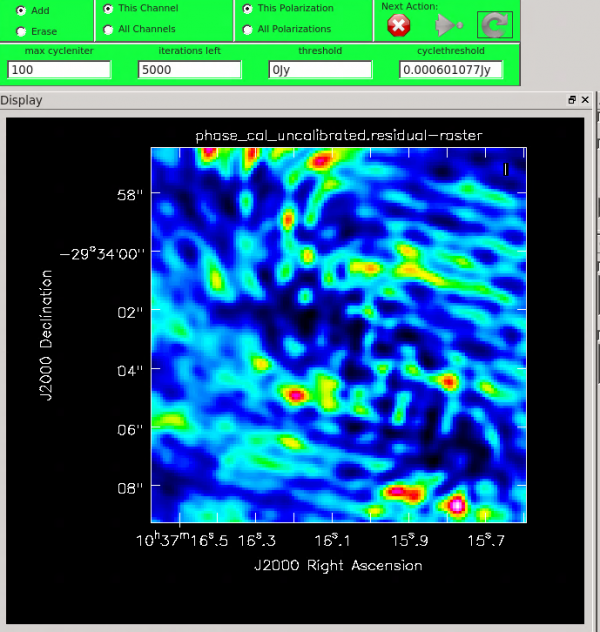
\includegraphics[width=0.8\textwidth]{Images/uncaliberated-image.png}
       \caption{Viewer image of the phase calibrator without any calibration.}
\end{figure}

\subsubsection{Effects of Unflagged Data}

\begin{lstlisting}[style=casa-python]
tclean(vis='sis14_twhya_calibrated.ms',
       imagename='phase_cal_unflagged',
       field='3',
       spw='',
       specmode='mfs',
       gridder='standard',
       deconvolver='hogbom',
       imsize=[128,128],
       cell=['0.1arcsec'],
       weighting='natural',
       threshold='0mJy',
       niter=5000,
       interactive=True)
\end{lstlisting}

\begin{figure}[H]
       \centering
       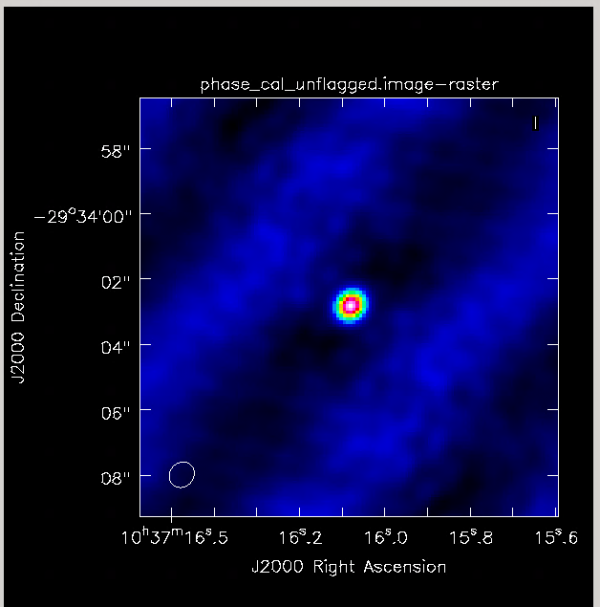
\includegraphics[width=0.8\textwidth]{Images/unflagged-image.png}
       \caption{Viewer image of the phase calibrator without any flagging of bad data.}
\end{figure}

\clearpage

\subsection{Continuum Image of TW Hydra}

\begin{lstlisting}[style=casa-python]
split(vis='sis14_twhya_calibrated_flagged.ms', field='5', width='8', outputvis='twhya_smoothed.ms', datacolumn='data')

tclean(vis='twhya_smoothed.ms',
       imagename='twhya_cont',
       field='0',
       spw='',
       specmode='mfs',
       gridder='standard',
       deconvolver='hogbom',
       imsize=[250,250],
       cell=['0.08arcsec'],
       weighting='briggs',
       robust=0.5,
       threshold='0mJy',
       niter=5000,
       interactive=True)
\end{lstlisting}

\begin{figure}[H]
       \centering
       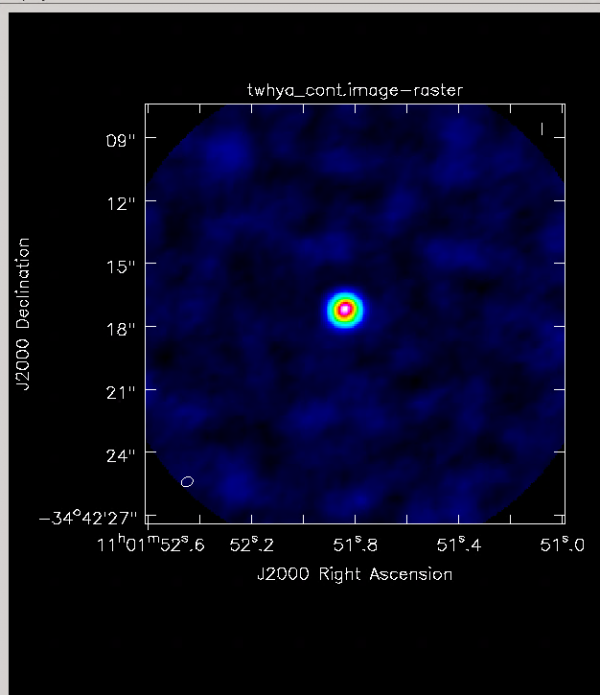
\includegraphics[width=0.7\textwidth]{Images/continuum-image.png}
       \caption{Continuum image for TW Hydra.}
\end{figure}

\clearpage

\subsection{Non-Interactive Cleaning Mode}

In the non-interactive mode of tclean, crucial parameters such as the threshold, mask, and maximum number of iterations play pivotal roles in controlling the deconvolution process. To set up tclean efficiently, first define a clean mask based on the regions of emission visible in the image. For instance, if emission is confined within a pixel range of $(100, 100)$ to $(150, 150)$, this box can be specified as the mask using the mask parameter. Alternatively, a mask file from an earlier interactive run can be used. Setting the stopping threshold involves estimating the noise level using tools like imview. In this scenario, an RMS noise of approximately $7$ mJy/beam suggests setting the threshold to about $15$ mJy/beam, which is twice the noise level. This approach helps to prevent the inclusion of random noise spikes as sources in the deconvolved image, thereby reducing false detections. \\

Additionally, the maximum number of iterations is set to $10,000$ as a failsafe measure. This high value ensures that tclean does not run indefinitely if something goes awry. The non-interactive mode of tclean offers a time-efficient and reproducible approach, though it is often advantageous to use the hybrid mode, starting interactively and then allowing tclean to continue automatically. This hybrid mode facilitates manual adjustments to the mask, threshold, and iteration parameters if necessary. For images with uncertain calibration or bright sources, an initial interactive cleaning process is recommended to ensure optimal results. Monitoring residuals during the cleaning cycles is essential, as increasing residuals may indicate the need for adjustments to the stopping threshold.

\vspace{15mm}

\begin{lstlisting}[style=casa-python]
tclean(vis='twhya_smoothed.ms',
       imagename='twhya_cont_auto',
       field='0',
       spw='',
       specmode='mfs',
       gridder='standard',
       deconvolver='hogbom',
       imsize=[250,250],
       cell=['0.08arcsec'],
       mask='box [ [ 100pix , 100pix] , [150pix, 150pix ] ]',
       weighting='briggs',
       robust=0.5,
       threshold='15mJy',
       niter=10000,
       interactive=False)
\end{lstlisting}
\chapter{Markov Chain Monte Carlo (MCMC)}

\section{Introduction}

In this section, we will discuss a powerful technique called Markov Chain Monte Carlo (MCMC) that is used to sample from the posterior distribution. MCMC is a class of algorithms that are used to sample from a probability distribution. The basic idea behind MCMC is to construct a Markov chain that has the desired distribution as its equilibrium distribution. The chain is then run for a large number of iterations and the samples generated are used to approximate the desired distribution. \\

The main advantage of MCMC is that it allows us to sample from complex, high-dimensional distributions that are difficult to sample from using other methods. MCMC is widely used in Bayesian statistics, machine learning, and other fields where sampling from complex distributions is required. \\

The idea is to compare generated samples with the target distribution and make small changes to the samples in order to make them more closely resemble the target distribution. This process is repeated until the samples are close enough to the target distribution. \\

\section{Markov Chains}

A Markov chain is a stochastic process that moves from one state to another according to a set of transition probabilities. The state of the chain at time $t$ is denoted by $X_t$, and the transition probabilities are denoted by $P(X_{t+1} | X_t)$. A Markov chain is said to be \textit{homogeneous} if the transition probabilities do not depend on time. \\

A Markov chain is defined by its state space, transition probabilities, and initial distribution. The state space is the set of all possible states that the chain can be in, and the transition probabilities specify the probability of moving from one state to another. The initial distribution specifies the probability of starting in each state. \\

A Markov chain is said to be \textit{irreducible} if it is possible to move from any state to any other state with positive probability. A Markov chain is said to be \textit{aperiodic} if the greatest common divisor of the lengths of all cycles in the chain is 1. A Markov chain that is both irreducible and aperiodic is said to be \textit{ergodic}. \\

An ergodic Markov chain has a unique stationary distribution, which is the distribution that the chain converges to as the number of iterations goes to infinity. The stationary distribution is also known as the equilibrium distribution or the limiting distribution. \\

\section{Fitting GW170817 Light Curve Data}

In this section, we will use MCMC to fit the light curve data from the GW170817 event. The light curve data consists of Observed Frequency and the flux density at each time step. We will use MCMC to sample from the posterior distribution of the parameters of the light curve model. \\

Light curves are graphical representations of the variation in brightness or flux of an astronomical object over time. Fitting light curves with models allows us to extract valuable information about the physical processes governing these sources. The smooth broken power-law model is one such model used to describe the flux evolution. \\

The light curve model is given by the following equation:

\begin{equation}
	F(t, \nu) = 2 ^ {\frac{1}{s}} \left(\dfrac{\nu}{3 \text{ GHz}}\right) ^ \beta \left[\left(\dfrac{t}{t_p} \right)^{-s \alpha_1} + \left(\dfrac{t}{t_p} \right)^{-s \alpha_2}\right] ^ {\frac{-1}{s}}
	\label{eq:smooth_broken_power_law}
\end{equation}

where:

\begin{itemize}
	\item $s$ is the spectral index.
	\item $F_p$ is the flux density at $3$ GHz at the light curve peak.
	\item $\beta$ is the spectral index.
	\item $t$ is the time post-merger.
	\item $t_p$ is the lightcurve peak time.
	\item $\alpha_1$ and $\alpha_2$ are the power-law rise and decay slopes respectively.
	\item $F(t, \nu)$ is the flux density at time $t$ and frequency $\nu$.
\end{itemize}

This is the initial Flux Density \textit{vs} Time data:

\begin{figure}[H]
	\centering
	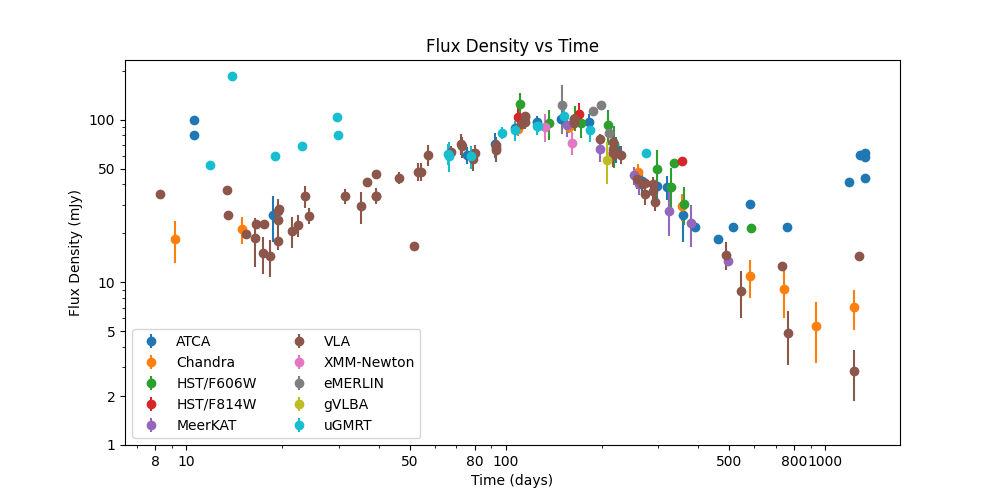
\includegraphics[width=\textwidth]{Images/FluxDensityvsTime.png}
	\caption{Flux Density \textit{vs} Time}
	\label{fig:flux_density_vs_time}
\end{figure}

And this is the corner plot which we get on running the MCMC Algorithm:

\begin{figure}[H]
	\centering
	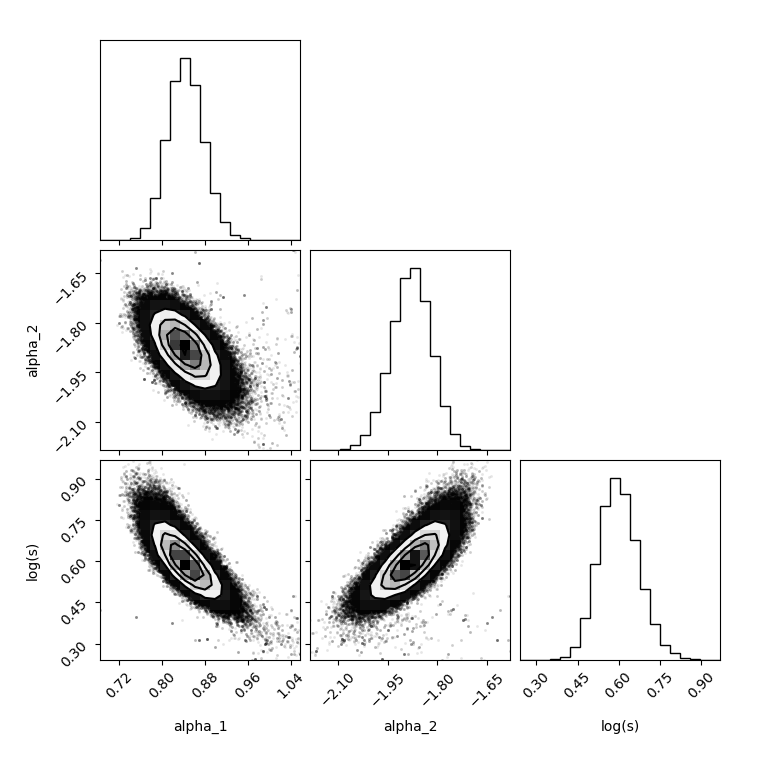
\includegraphics[width=\textwidth]{Images/corner_plot.png}
	\caption{Corner Plot}
	\label{fig:corner_plot}
\end{figure}

\clearpage

Finally this is the best fit light curve model:

\begin{figure}[H]
	\centering
	\includegraphics[width=\textwidth]{Images/Best_fit_model.png}
	\caption{Best Fit Light Curve Model}
	\label{fig:light_curve_model}
\end{figure}

Running MCMC for all parameters raised the \verb|WARNING:root:Too few points to create valid contours|, so I decided to run MCMC for only 3 parameters at a time. The corner plot shows the posterior distribution of the parameters, and the best fit light curve model is shown in the last figure.




\nocite{*}
\bibliographystyle{alpha}
\bibliography{references}
\addcontentsline{toc}{chapter}{Bibliography}

\end{document}
